\chapter{Searching for an \textit{(un)stable equilibrium}:
Experiments in Training Generative Neural Networks Without Data}
\label{ch:unstable_eq}

\section{Introduction}

This chapter details the first successful attempt in my PhD research in finding a way of training a generative neural network in a data divergent (or data agnostic) way. 
This work is one of the first recorded endeavours of training a generative neural network without training data, alongside Joel Simon’s excellent work Dimensions of dialogue [\citeyear{simon2019dimensions}, and was the first published and peer-reviewed publication on training generative neural networks without data.
These works were done concurrently and independently of each other, and were disseminated at around the same time \footnote{Joel Simons Blog does not contain a date, so I cannot determine an exact chronology here}. 

This work was published as a short paper at the NerIPS 2019 Workshop on Machine Learning for Creativity and Design, in Vancouver, Canada \citep{broad2019searching}. 
Chapter \ref{ch:impact} details the reception of the series of artworks \textit{(un)stable equilibrium} that resulted from these experiments. 

In that initial paper I documented 6 experiments, each training run become the artworks \textit{(un)stable equilibrium 1:1} through to \textit{(un)stable equilibrium 1:6} (Figure \ref{fig:c3:original-experiments}). Unfortunately due to time, entropy and multiple computer and disk-drive failures, I have lost the original logs and training samples from these initial training run samples. Therefore the rest of the results presented in this paper of experiments are re-runs of the original experiments (as faithfully as I could make them). The results are similiar, but not identical to the ones in the original paper, as it was not possible to perfectly replicate these original experiments without the same initial training parameters, hyperparameters and sampling schedule. \S \ref{c7:sec:unstable_eq} details the reception and artistic presentation of the original training runs in more detail. 

\begin{figure}[!htbp]
    \centering
    \subfloat[]{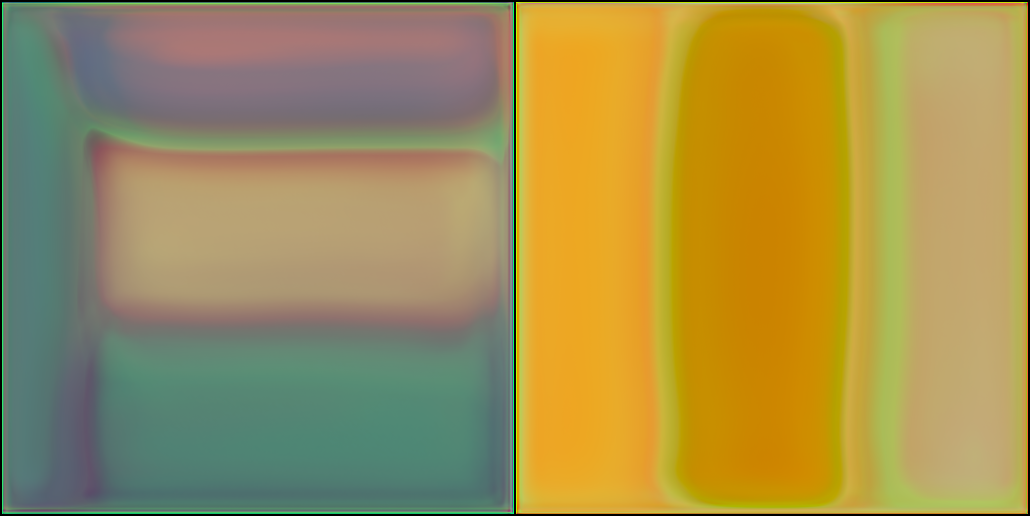
\includegraphics[width=0.45\textwidth]{figures/c4_unstable/original_experiments/1_1.png}}
    \hfill
    \subfloat[]{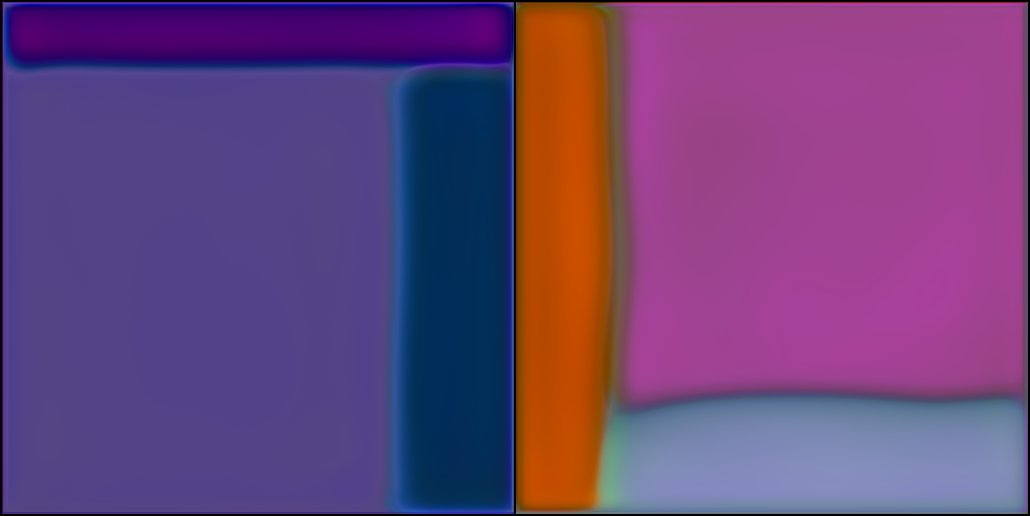
\includegraphics[width=0.45\textwidth]{figures/c4_unstable/original_experiments/1_2.png}}
    \hfill
    \subfloat[]{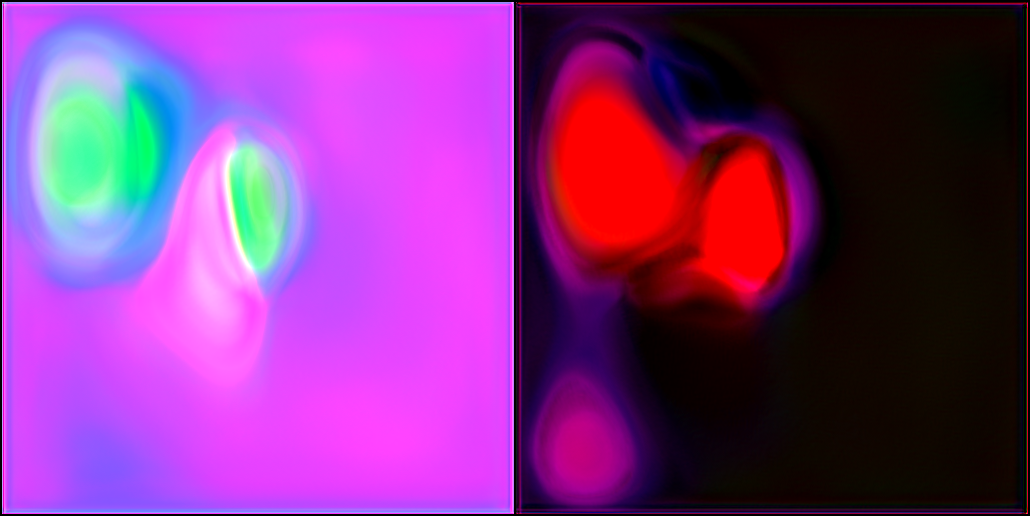
\includegraphics[width=0.45\textwidth]{figures/c4_unstable/original_experiments/1_3.png}}
    \hfill
    \subfloat[]{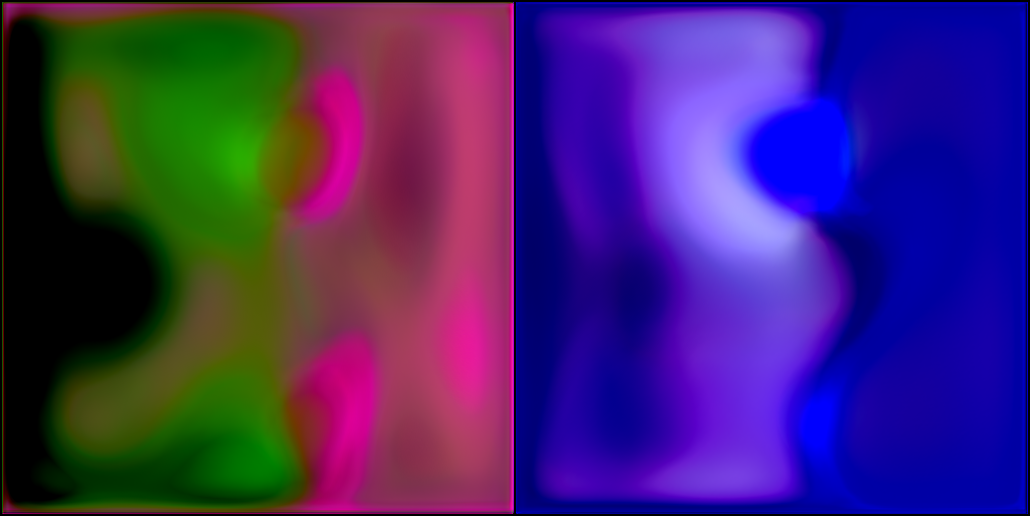
\includegraphics[width=0.45\textwidth]{figures/c4_unstable/original_experiments/1_4.png}}
    \hfill
    \subfloat[]{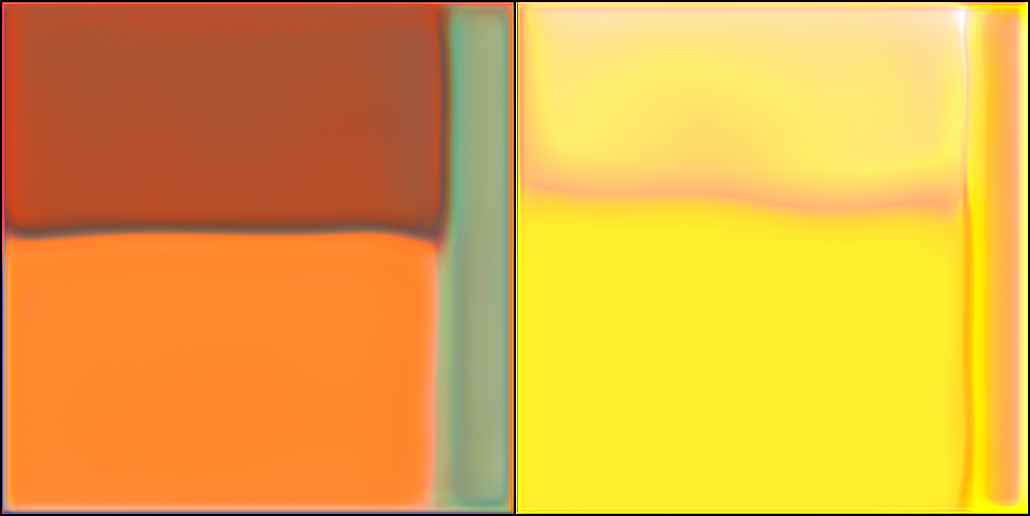
\includegraphics[width=0.45\textwidth]{figures/c4_unstable/original_experiments/1_5.png}}
    \hfill
    \subfloat[]{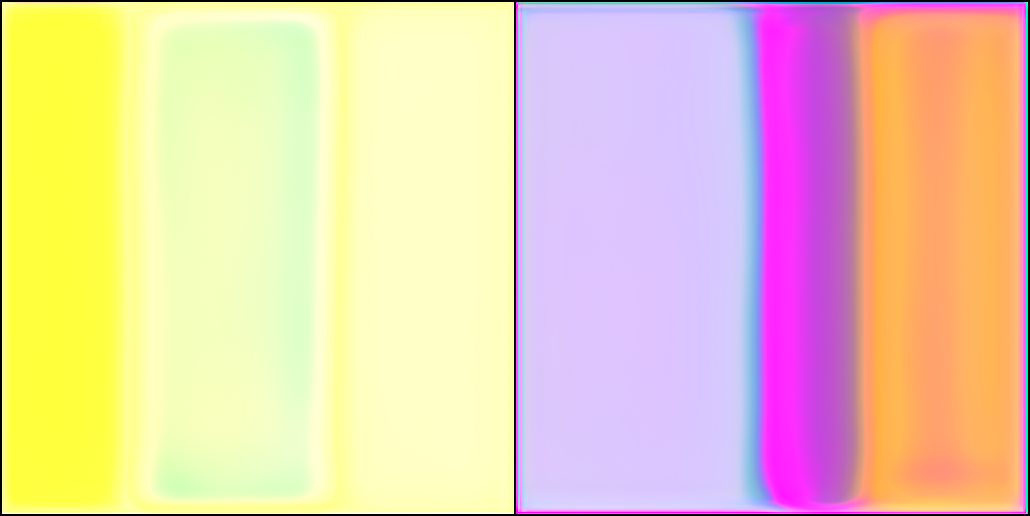
\includegraphics[width=0.45\textwidth]{figures/c4_unstable/original_experiments/1_6.png}}
    \caption[Original experiments in the \textit{(un)stable equilibrium} series]{Original experiments in the \textit{(un)stable equilibrium} series. (a) \textit{(un)stable equilibrium 1:1}, (b) \textit{(un)stable equilibrium 1:2}, (c) \textit{(un)stable equilibrium 1:3}, (d) \textit{(un)stable equilibrium 1:4}, (e) \textit{(un)stable equilibrium 1:5}, (f) \textit{(un)stable equilibrium 1:6}.}
    \label{fig:c3:original-experiments}
  \end{figure}

\section{Motivation}

This work came out of a deep frustration early on in my PhD journey, where I was trying to find ways of training generative models without modelling data.
It took me far longer than it should have to come to the realisation that this is an oxymoron. 
That a generative model is a model of a data distribution, and nothing more. 
Any attempt to move past this notion needed a completely different approach, and the first approach I developed which was fruitful is what is presented in this chapter. 

This work came out of a simple proposition: if it was possible to find a way of training a generative neural network without any training data, then by default, any outcome must be novel and could not resemble an existing training data distribution. 
There was little mathematical grounding to this approach. 
Through dogged trial and error, some playful reconfiguring of the most common (at the time) way of training generative models, GANs, I was able to find a way to train generative networks without data, in ways that produced at the very least, aesthetically interesting outcomes. 

This chapter tells the story of that process. 
Through the early experiments with configurations of models and loss functions that led to unremarkable results, through to the final configuration of models and training runs that resulted in the artworks \textit{(un)stable equilibrium}.
This chapter is named as such, because the journey I went on in producing those works was one of searching -- through intuition and aesthetic exploration -- for an (un)stable equilibrium. 
A balancing act of finding a system just chaotic enough to produce enough randomness in the resulting training run that enough unpredictable dynamics would lead to configuration of the weight parameters of the model such that unpredictable (and aesthetically compelling) results would come from the generator networks. 
But not enough for the loss functions to explode during training. 
The visual results of training were monitored, both visually by me as I inspected the generated output as each training increment progressed, along with a close monitoring of the fluctuations of the various loss functions throughout training. 
Over the course of a couple of intensive weeks of working in this unorthodox way, the configuration that produced these results was discovered. 

\section{Initial experiments}

My first experiment took inspiration from the GAN framework (Figure \ref{subfig:c3:og-gan-diagram}) where a generator network imitates a training dataset, and the discriminator tries to tell them apart (Eq. \ref{eq:gan-loss}). 

\begin{equation} 
    Adv =\min_{G}\max_{D}\mathbb{E}_{x\sim p_{\text{data}}(x)}[\log{D(x)}])+  \mathbb{E}_{z\sim p_{\text{z}}(z)}[1 - \log{D(G(z))}]
    \label{eq:gan-loss}
\end{equation}

My initial adaptation of this was to replace the training data with another generator (Figure \ref{subfig:c3:double-gen-diagram}). 
In this arrangement the two discriminators are trying to imitate each other, whilst the discriminator is still trying to tell them apart (Eq. \ref{eq:double-gen-gan-loss}).

\begin{equation} 
    Adv = \min_{G_{1}}\max_{G_2}\max_{D}\mathbb{E}_{x\sim p_{\text{data}}(x)}[\log{D(x)}] +  \mathbb{E}_{z\sim p_{\text{z}}(z)}[1 - \log{D(G(z))}]
    \label{eq:double-gen-gan-loss}
\end{equation}

\begin{figure}[!htbp]
    \centering
    \subfloat[]{\label{subfig:c3:og-gan-diagram}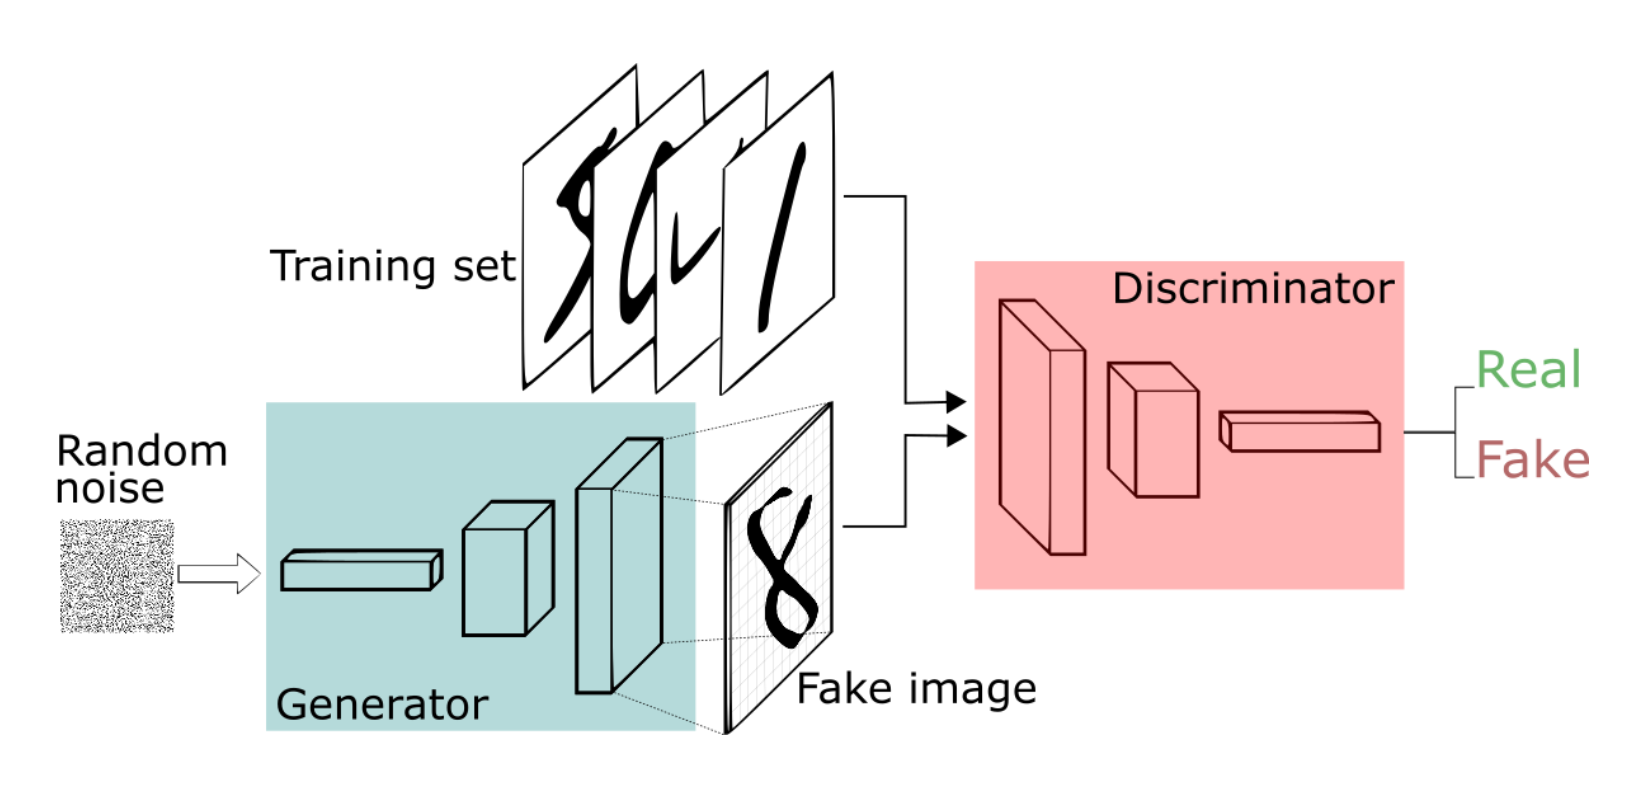
\includegraphics[width=0.75\textwidth]{figures/c4_unstable/diagrams/gan.png}}
    \hfill
    \subfloat[]{\label{subfig:c3:double-gen-diagram}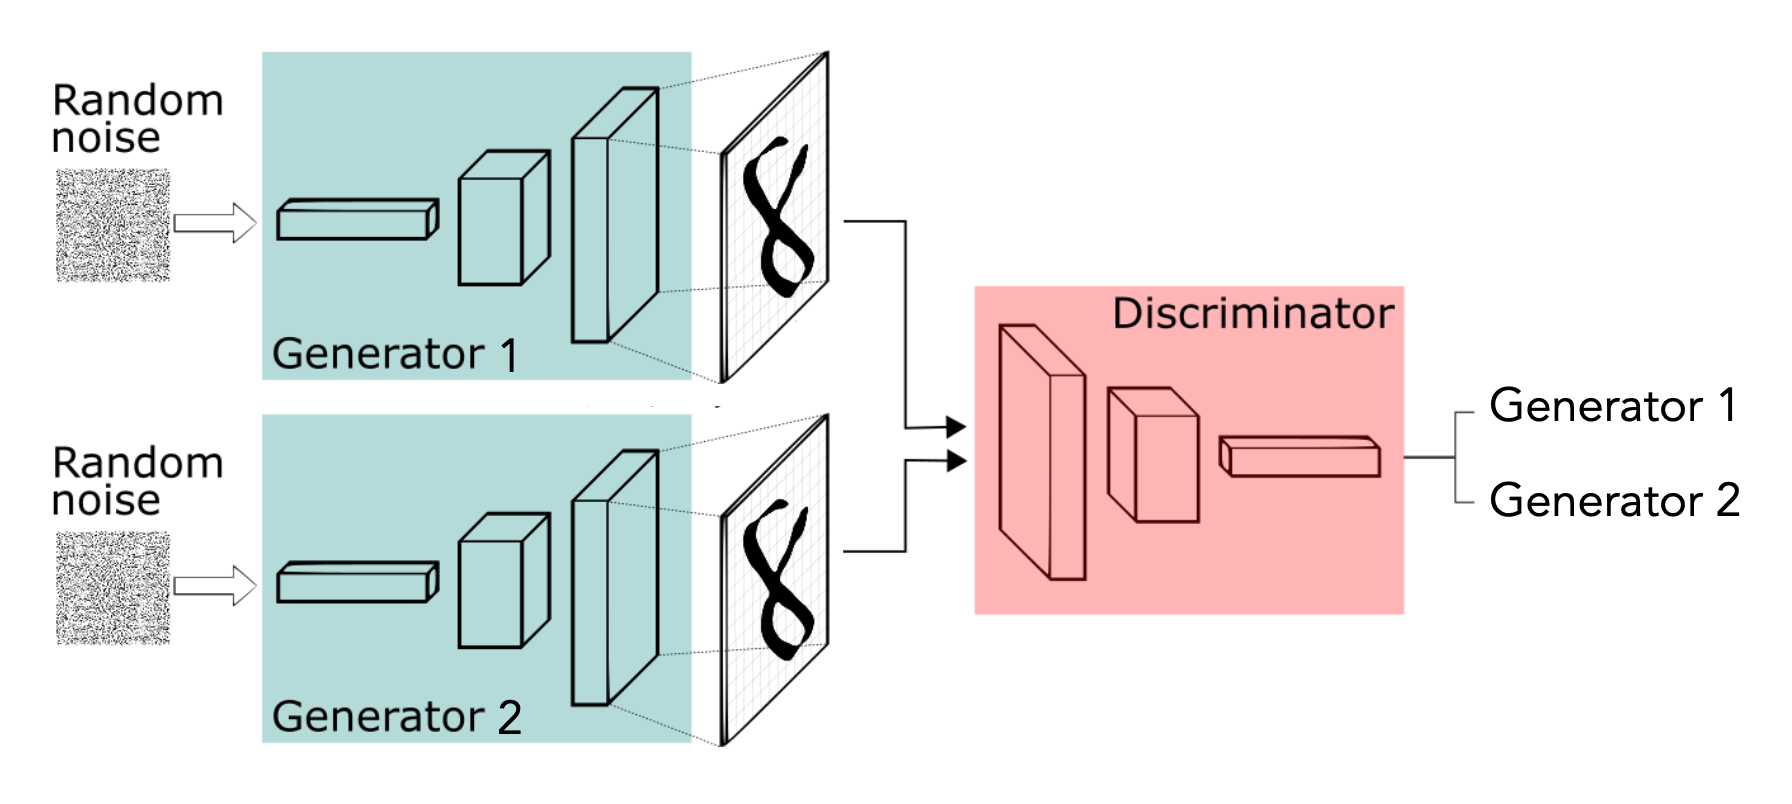
\includegraphics[width=0.75 \textwidth]{figures/c4_unstable/diagrams/two-generator.png}}
    \caption[GAN architecture training diagrams]{GAN architecture training diagrams. (a) The original GAN training framework where one generator imitates training data \citep{goodfellow2014generative}. (b) Novel training architecture where the training data is replaced with another generator in order to train two generative neural networks without data.}
    \label{fig:c3:gan-diagrams}
  \end{figure}

\subsection{Adversarial loss}

Figures \ref{fig:c3:samples-no-col-var} \& \ref{fig:c3:no-var-losses} show the samples during training and loss logs during training respectively.
These, and all following experiments were done with a batch size of 10. 

\textbf{Add all other training parameters here}

\label{c4:sec:og-loss}

\FloatBarrier
\begin{figure}[!htbp]
    \centering
    \subfloat[]{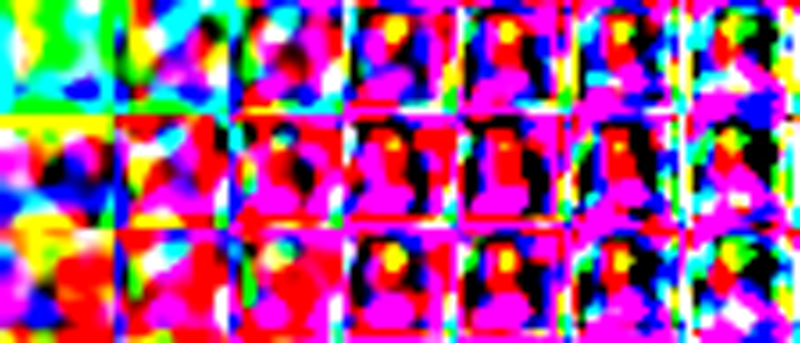
\includegraphics[width=0.45\textwidth]{figures/c4_unstable/train_samples/no_col_var/scaled_step_2_g1.png}}
    \hfill
    \subfloat[]{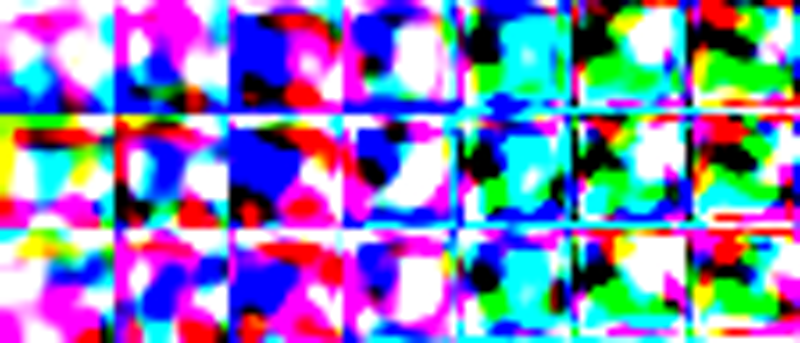
\includegraphics[width=0.45\textwidth]{figures/c4_unstable/train_samples/no_col_var/scaled_step_2_g2.png}}
    \hfill
    \subfloat[]{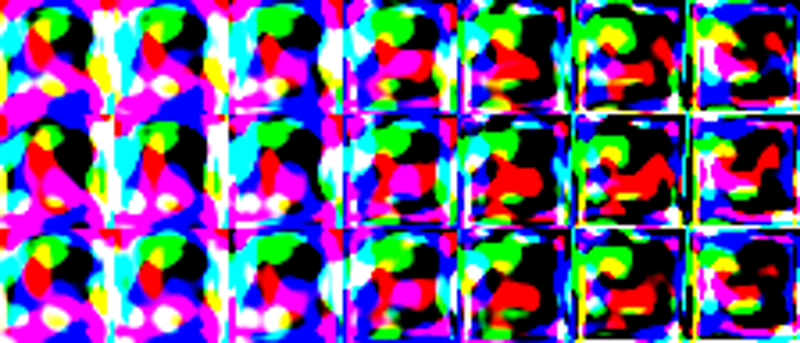
\includegraphics[width=0.45\textwidth]{figures/c4_unstable/train_samples/no_col_var/scaled_step_3_g1.png}}
    \hfill
    \subfloat[]{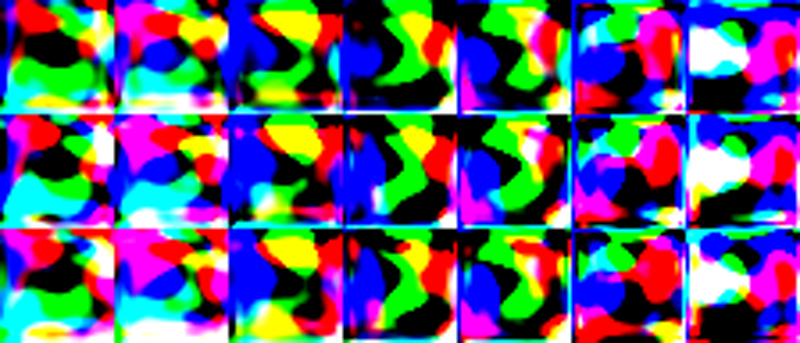
\includegraphics[width=0.45\textwidth]{figures/c4_unstable/train_samples/no_col_var/scaled_step_3_g2.png}}
    \hfill
    \subfloat[]{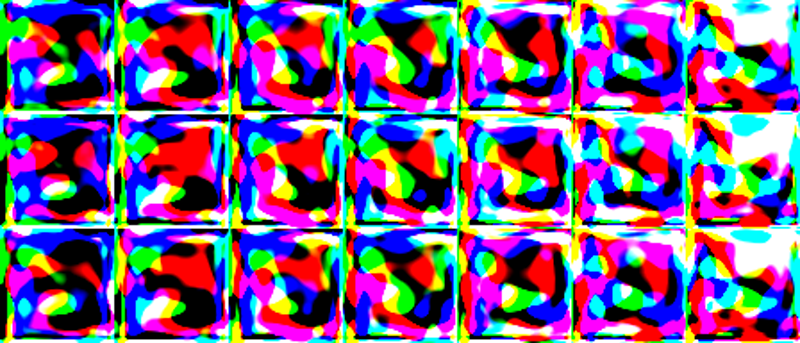
\includegraphics[width=0.45\textwidth]{figures/c4_unstable/train_samples/no_col_var/scaled_step_4_g1.png}}
    \hfill
    \subfloat[]{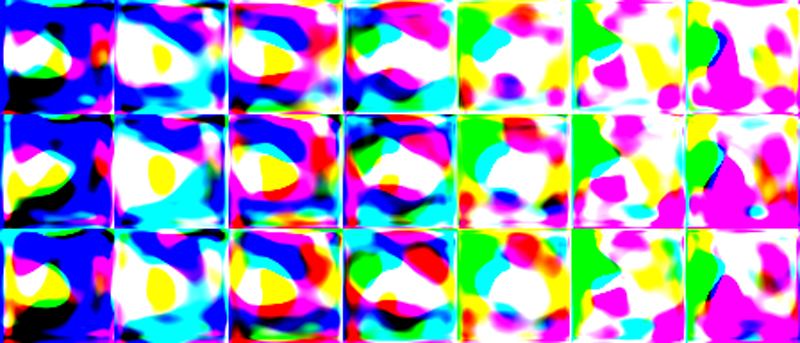
\includegraphics[width=0.45\textwidth]{figures/c4_unstable/train_samples/no_col_var/scaled_step_4_g2.png}}
    \hfill
    \subfloat[]{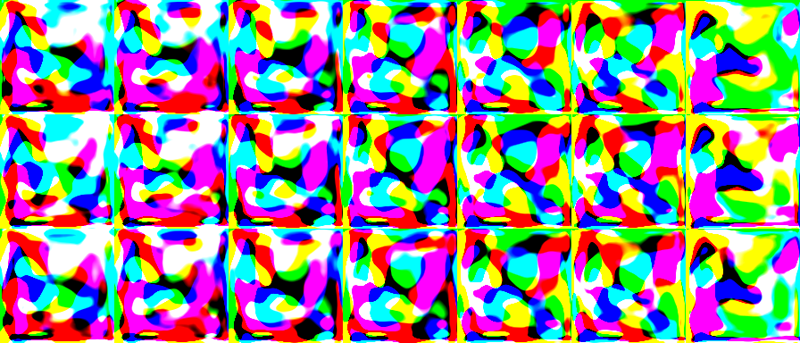
\includegraphics[width=0.45\textwidth]{figures/c4_unstable/train_samples/no_col_var/scaled_step_5_g1.png}}
    \hfill
    \subfloat[]{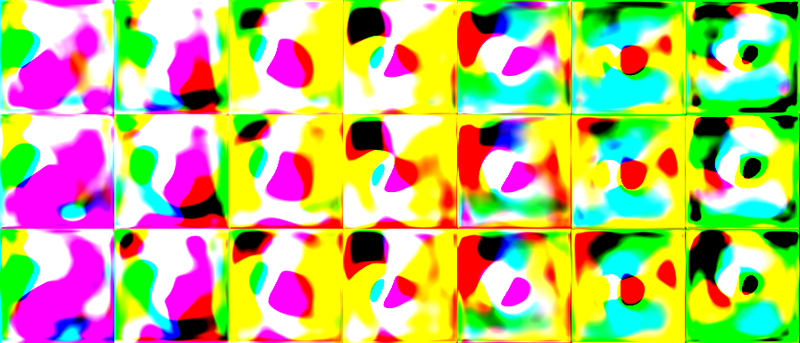
\includegraphics[width=0.45\textwidth]{figures/c4_unstable/train_samples/no_col_var/scaled_step_5_g2.png}}
    \hfill
    \subfloat[]{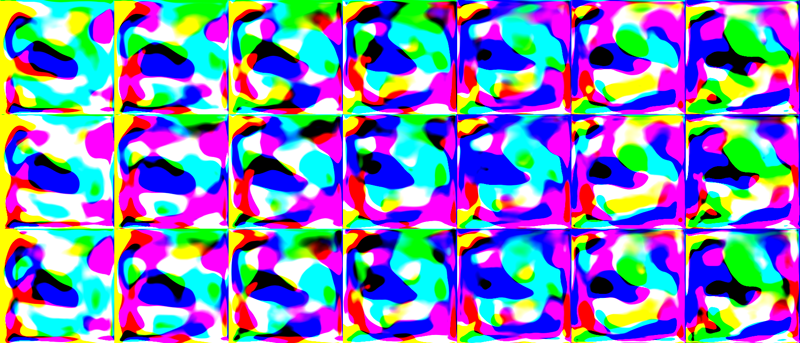
\includegraphics[width=0.45\textwidth]{figures/c4_unstable/train_samples/no_col_var/scaled_step_6_g1.png}}
    \hfill
    \subfloat[]{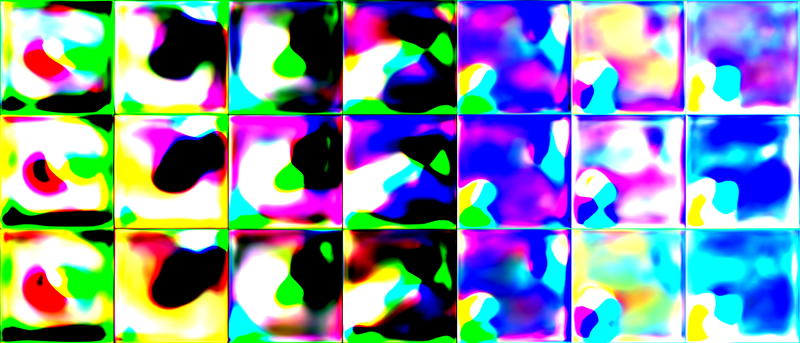
\includegraphics[width=0.45\textwidth]{figures/c4_unstable/train_samples/no_col_var/scaled_step_6_g2.png}}
    \hfill
    \caption[Training samples for standard adversarial training with two generators]{Training samples for standard adversarial training with two generators, sampled at increments of 50 iterations. The left column shows the training samples for $G_{1}$ and the right column shows the trianing samples for $G_{2}$. (a,b) Training samples at resolution 32x32 for iterations 0-300. (c,d) Training samples at resolution 64x64 for iterations 300-600. (e,f) Training samples at resolution of 128x128 for iterations 600-900. (g,h) Training samples at resolution 256x256 at iterations 900-1200. (i,j) Training samples at resolution 512x512 for iterations 1200-1500.}
    \label{fig:c3:samples-no-col-var}
  \end{figure}

  \begin{figure}[!htbp]
    \centering
    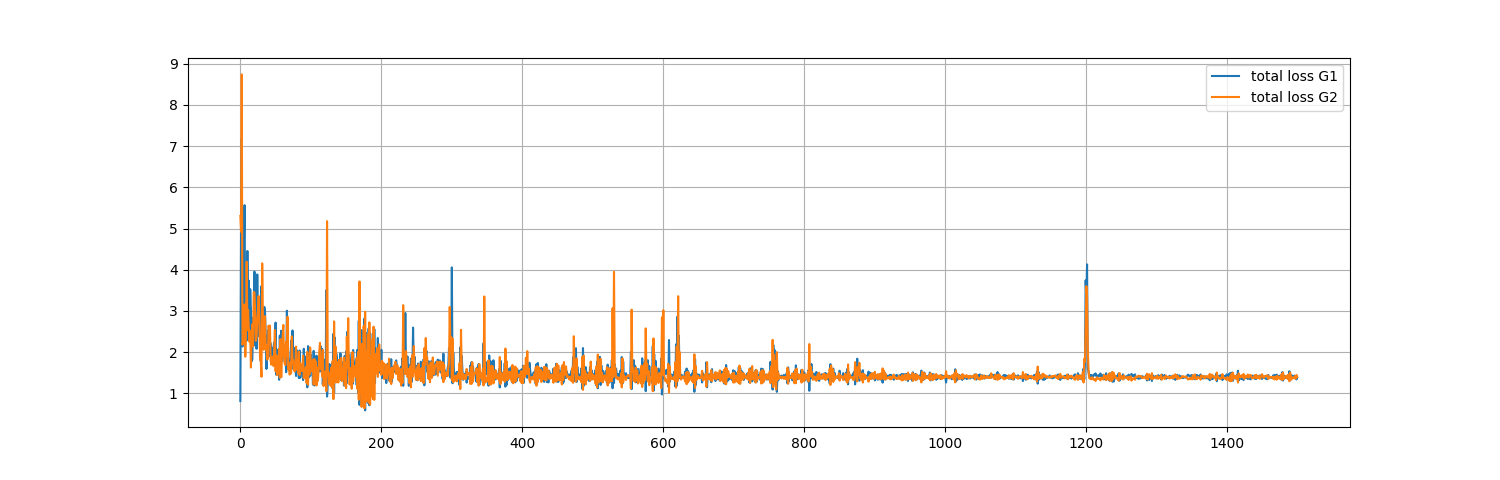
\includegraphics[width=1\textwidth]{figures/c4_unstable/train_losses/no_col_var/total_loss_no_var.png}
    \caption[Loss plot for double adversarial training]{Loss plot for double adversarial training of the two generator networks. Note: the loss for the discriminator is the same as the second generator.}
  \label{fig:c3:no-var-losses}
  \end{figure}

In this setting the visual results (Figure \ref{fig:c3:samples-no-col-var}) were not what I was hoping for.  
There is little diversity across the training batch for both generators. 
Essenitally, this training regime has suffered from mode collapse, which is a common failure state for GANs where the generator collapses into generating a single output in the output data distribution. 

In the normal GAN training regime, this diversity in the output images comes from mimicking the training data, which should have a wide variety of data samples in it (aka modes). 
Without training data, it is not surpirsing then that these models quickly collapse to a single mode of generation for each of the respective generators. 
To overcome this I needed to add an additional term to force to model into producing more diverse outputs. 
This is detailed in the following subsection.

\subsection{Colour variance loss term}

In response to the mode collapse suffered in the previous experiment I developed an additional loss function to the training regime of this two generator training regime.
The additional loss term was designed to force increased colours to be used was to measure the batch-wide variance of values for each pixel, in each channel of the tensor. 
This term calculates the variance across the sampled batch $B$ for the respective channel c of the tensor for the samples drawn from both generators $g_{1}$ and $g_{2}$, which are then subtracted from each other (depending on which loss is being calculated for which generator) to enforce a relative variance that is higher than the other model across the different channels of the sample tensor.

\begin{equation}
    \label{eq:variance-gan}
    Vdiff = Var(B_{g_{1}}^{c}) - Var(B_{g_{2}}^{c})
    \end{equation}

This is calculated for the 4 channels of the tensor present in the sample batch. 
The first channel is the overall batch bt, the following channels are the colour channels of the output images: red r, green g and blue b.

\begin{equation}
    \label{eq:total-gan}
        Vdiff(B_{g_{1}}^{bt} , B_{g_{2}}^{bt}) + Vdiff(B_{g_{1}}^{r} , B_{g_{2}}^{r}) + Vdiff(B_{g_{1}}^{g} , B_{g_{2}}^{g}) +  dVdiff(B_{g_{1}}^{b} , B_{g_{2}}^{b}) 
    \end{equation}

The loss penalty was calculated for each generator with respect to the other. 
Therefore each generator was optimised to have more mini-batch variance than the other. 
Adding this term made a significant impact to the training. Eq. \ref{eq:gan-g1-col-var} shows the training objective for $G_{1}$ and Eq.  \ref{eq:gan-g2-col-var} shows the training objective for $G_{2}$.

\begin{equation} 
    G_{1}\ loss = \min_{G_{1}}Adv + Var(B_{g_{1}}^{c}) - Var(B_{g_{2}}^{c})
    \label{eq:gan-g1-col-var}
\end{equation}

\begin{equation} 
    G_{2}\ loss = \max_{G_{2}}Adv + Var(B_{g_{2}}^{c}) - Var(B_{g_{1}}^{c})
    \label{eq:gan-g2-col-var}
\end{equation}

Figures \ref{fig:c3:samples-col-var} \& \ref{fig:c3:col-var-losses} show the samples during training and loss logs during training respectively.

\begin{figure}[!htbp]
    \centering
    \subfloat[]{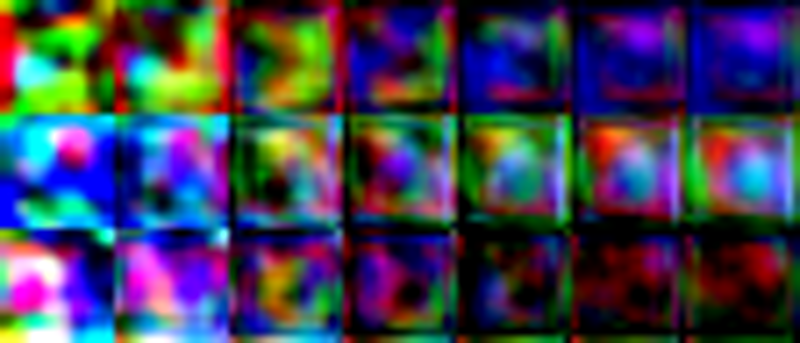
\includegraphics[width=0.45\textwidth]{figures/c4_unstable/train_samples/col_var/scaled_step_2_g1.png}}
    \hfill
    \subfloat[]{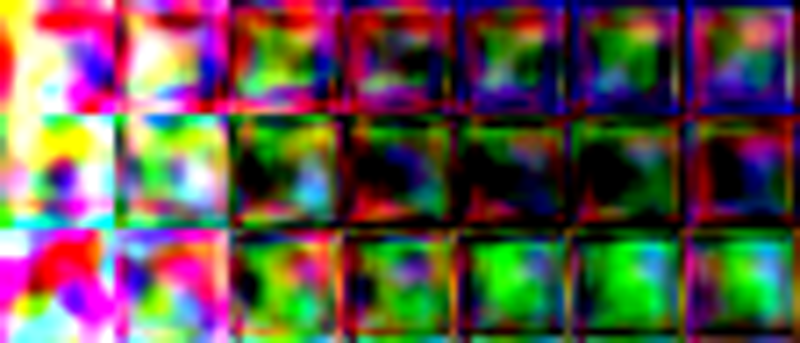
\includegraphics[width=0.45\textwidth]{figures/c4_unstable/train_samples/col_var/scaled_step_2_g2.png}}
    \hfill
    \subfloat[]{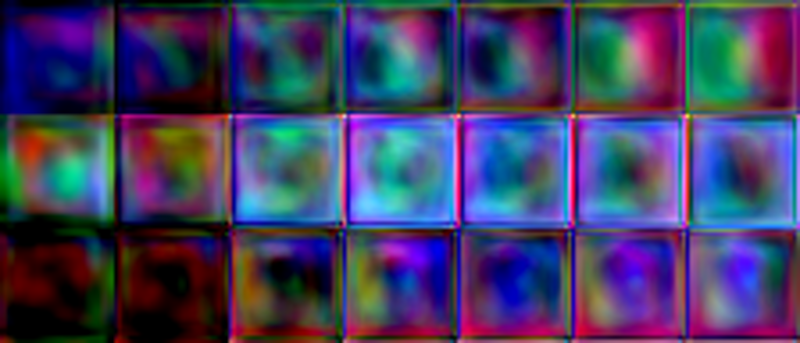
\includegraphics[width=0.45\textwidth]{figures/c4_unstable/train_samples/col_var/scaled_step_3_g1.png}}
    \hfill
    \subfloat[]{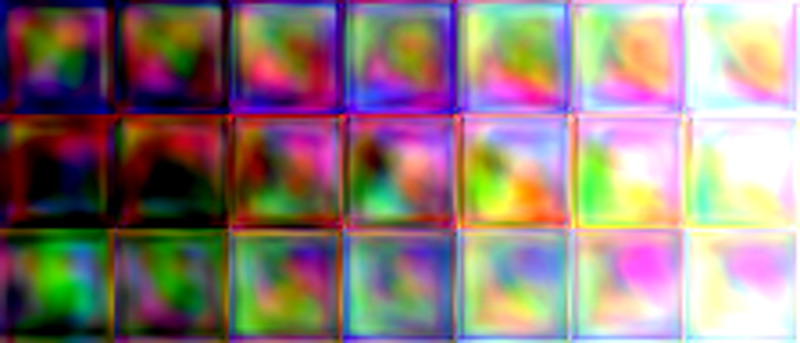
\includegraphics[width=0.45\textwidth]{figures/c4_unstable/train_samples/col_var/scaled_step_3_g2.png}}
    \hfill
    \subfloat[]{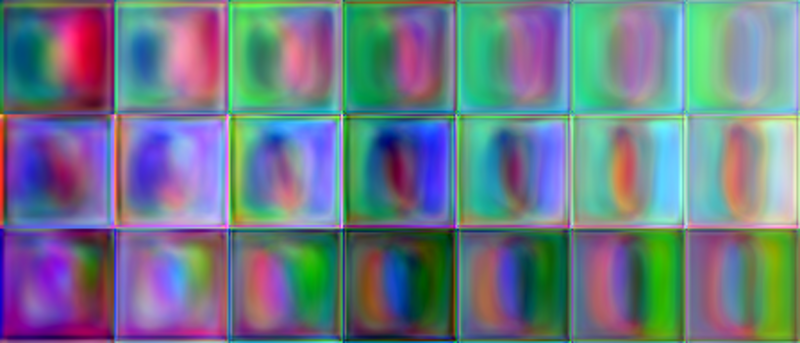
\includegraphics[width=0.45\textwidth]{figures/c4_unstable/train_samples/col_var/scaled_step_4_g1.png}}
    \hfill
    \subfloat[]{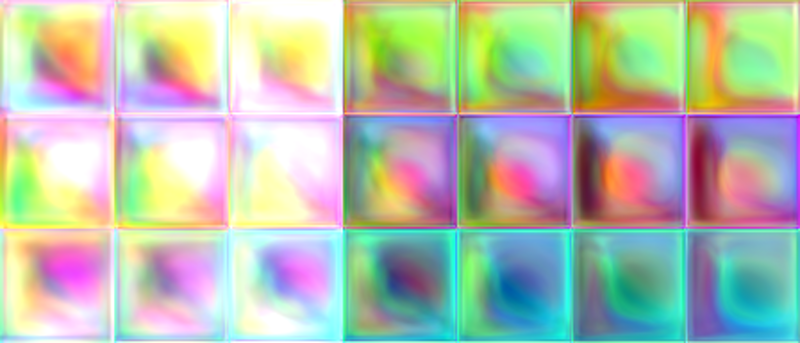
\includegraphics[width=0.45\textwidth]{figures/c4_unstable/train_samples/col_var/scaled_step_4_g2.png}}
    \hfill
    \subfloat[]{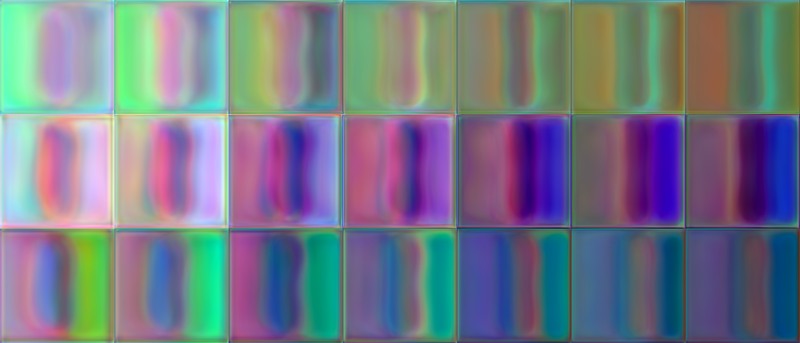
\includegraphics[width=0.45\textwidth]{figures/c4_unstable/train_samples/col_var/scaled_step_5_g1.png}}
    \hfill
    \subfloat[]{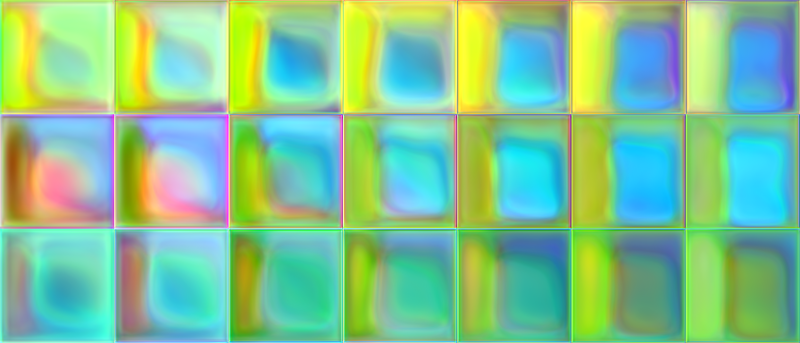
\includegraphics[width=0.45\textwidth]{figures/c4_unstable/train_samples/col_var/scaled_step_5_g2.png}}
    \hfill
    \subfloat[]{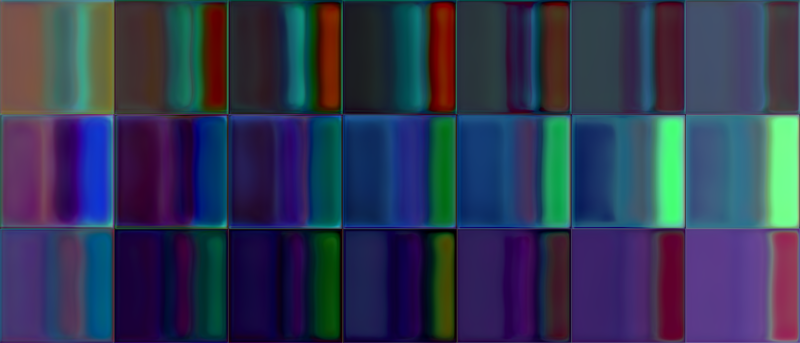
\includegraphics[width=0.45\textwidth]{figures/c4_unstable/train_samples/col_var/scaled_step_6_g1.png}}
    \hfill
    \subfloat[]{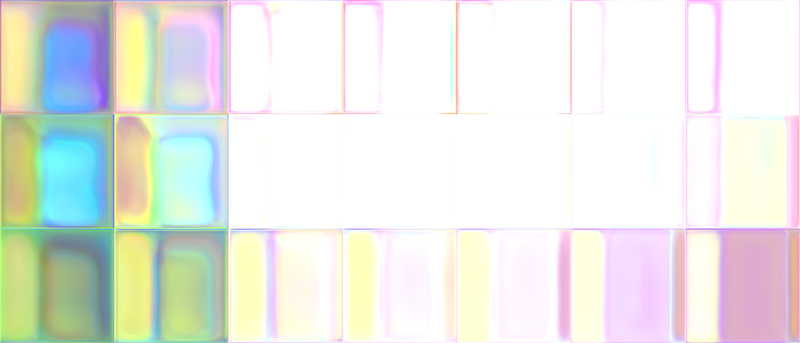
\includegraphics[width=0.45\textwidth]{figures/c4_unstable/train_samples/col_var/scaled_step_6_g2.png}}
    \hfill
    \caption[Training samples for adversarial training with two generators with the colour variance loss]{Training samples for adversarial training with two generators with the colour variance loss, sampled at increments of 50 iterations. The left column shows the training samples for $G_{1}$ and the right column shows the trianing samples for $G_{2}$. (a,b) Training samples at resolution 32x32 for iterations 0-300. (c,d) Training samples at resolution 64x64 for iterations 300-600. (e,f) Training samples at resolution of 128x128 for iterations 600-900. (g,h) Training samples at resolution 256x256 at iterations 900-1200. (i,j) Training samples at resolution 512x512 for iterations 1200-1500.}
    \label{fig:c3:samples-col-var}
  \end{figure}

  \begin{figure}[!htbp]
    \centering
    \subfloat[]{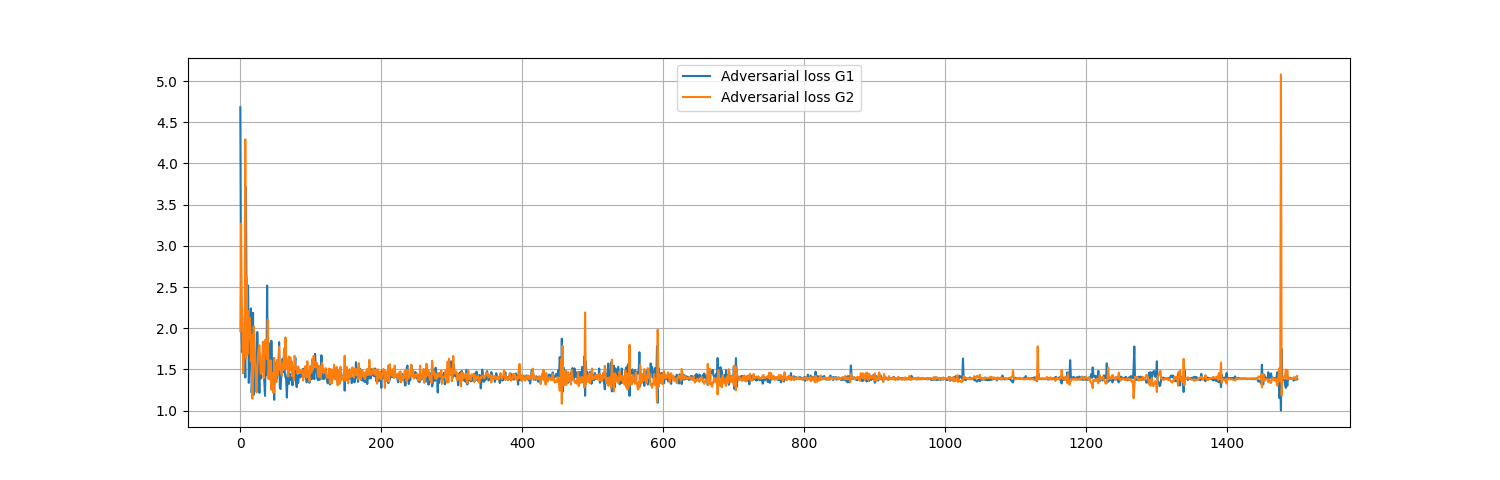
\includegraphics[width=1\textwidth]{figures/c4_unstable/train_losses/col_var/adversarial_loss.png}}
    \hfill
    \subfloat[]{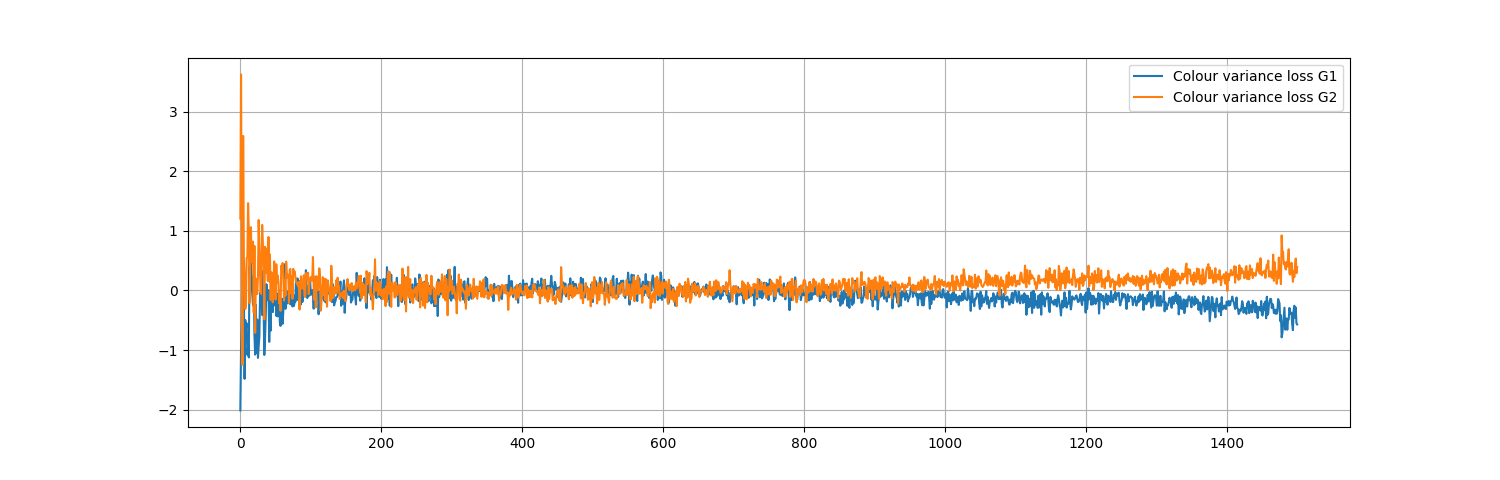
\includegraphics[width=1\textwidth]{figures/c4_unstable/train_losses/col_var/col_var_loss.png}}
    \hfill
    \subfloat[]{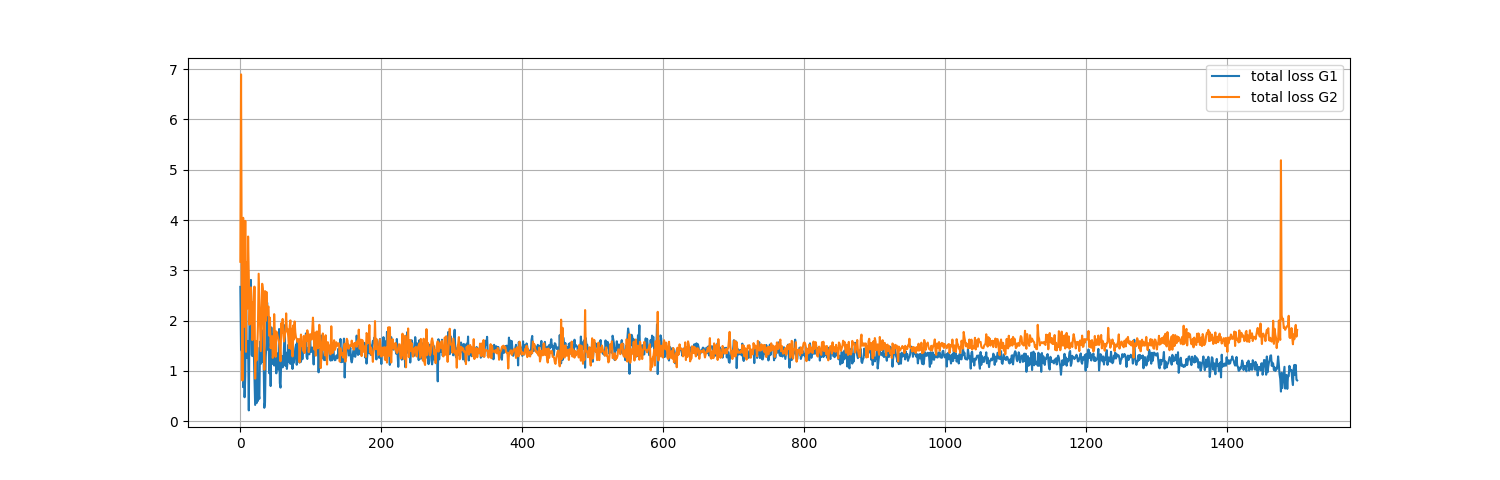
\includegraphics[width=1\textwidth]{figures/c4_unstable/train_losses/col_var/total_loss.png}}
    \caption[Loss plot for double adversarial training with colour variation loss term]{Loss plot for double adversarial training with colour variation loss term. (a) Advesarial loss terms for both respective generators. (b) Colour variation loss term for both respective generators. (c) Total loss combining both terms for both respective generators. }
    \label{fig:c3:col-var-losses}
  \end{figure}

\FloatBarrier

The visual results (Figure \ref{fig:c3:samples-col-var}) with this additional loss term show much improvement in respect to the variety across the generated data distribution, with respect to the previous experiment without the colour variance loss term (Figure \ref{fig:c3:samples-no-col-var}).
Whilst the visual results are simple in their composition, there is variety in colours generated across the generative space of both generators, which is exactly what I had been intending would happen with this additional loss term. 

In the following experiments I take these experiments further, keeping the colour diversity loss term, but replacing the adversarial loss terms with other means of measure distance and difference using common loss functions from metric learning. 
  
\section{Distance functions as alternatives to adversarial loss}

In these further experiments I replace the adversarial loss with other means of measuring difference and distance using two common loss functions in machine learning, that come from metric learning. 
To calculate these losses efficiently the discriminator is kept in place, but here the discriminator network is used to calculate feature vector embeddings of each of the generated samples.
Pair-wise distances are calculated per-generated sample from the respective generators, where both generators are sampled using the same fixed latents during training.
The two pairwise distance loss functions used are the cosine distance and Euclidean distance, which are detailed in the following two subsections.

\subsection{Cosine distance}

\begin{equation} 
    Cosine\ distance(x,y) = 1 - \frac{x \cdot y}{|x||y|}
    \label{eq:cosine-dist}
\end{equation}

\begin{equation} 
    G_{1}\ loss = 1 - \frac{\vec g_{1} \cdot \vec g_{2}}{|\vec g_{1}||\vec g_{2}|} + Var(B_{g_{1}}^{c}) - Var(B_{g_{2}}^{c})
    \label{eq:g1-cosine-loss}
\end{equation}

\begin{equation} 
    G_{2}\ loss = 1 - \frac{\vec g_{2} \cdot \vec g_{1}}{|\vec g_{2}||\vec g_{1}|} + Var(B_{g_{2}}^{c}) - Var(B_{g_{1}}^{c})
    \label{eq:g2-cosine-loss}
\end{equation}

\FloatBarrier

\begin{figure}[!htbp]
    \centering
    \subfloat[]{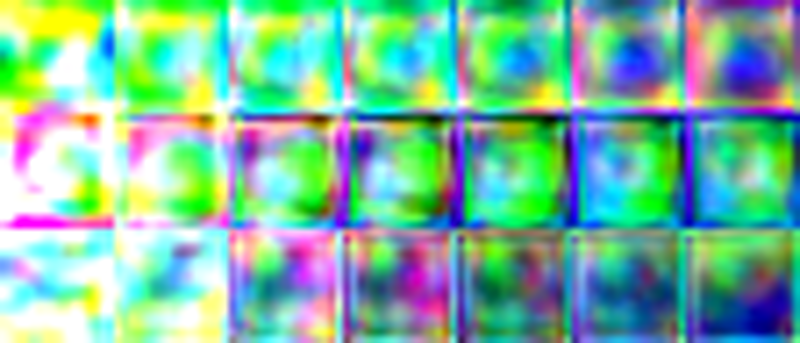
\includegraphics[width=0.45\textwidth]{figures/c4_unstable/train_samples/cos_cos/scaled_step_2_g1.png}}
    \hfill
    \subfloat[]{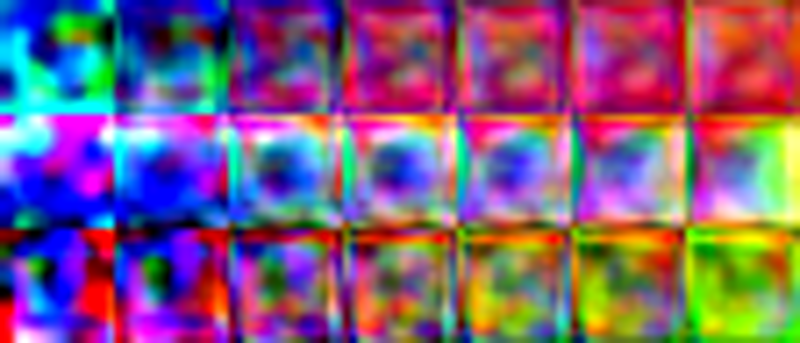
\includegraphics[width=0.45\textwidth]{figures/c4_unstable/train_samples/cos_cos/scaled_step_2_g2.png}}
    \hfill
    \subfloat[]{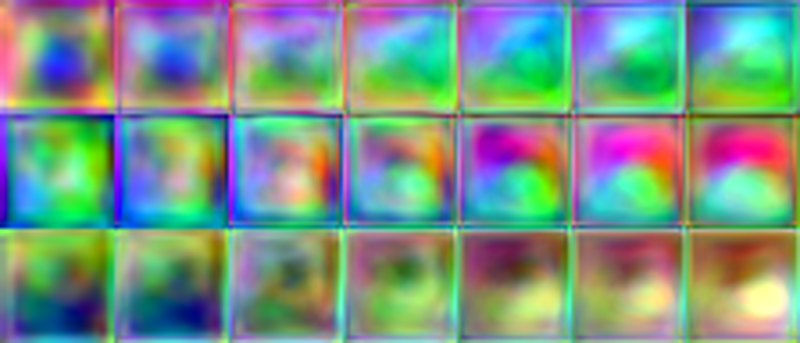
\includegraphics[width=0.45\textwidth]{figures/c4_unstable/train_samples/cos_cos/scaled_step_3_g1.png}}
    \hfill
    \subfloat[]{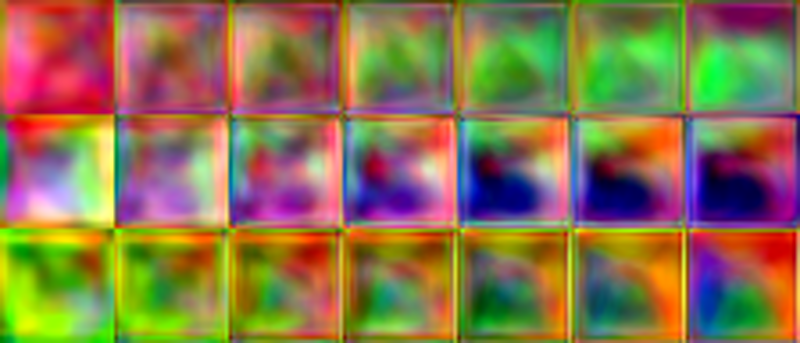
\includegraphics[width=0.45\textwidth]{figures/c4_unstable/train_samples/cos_cos/scaled_step_3_g2.png}}
    \hfill
    \subfloat[]{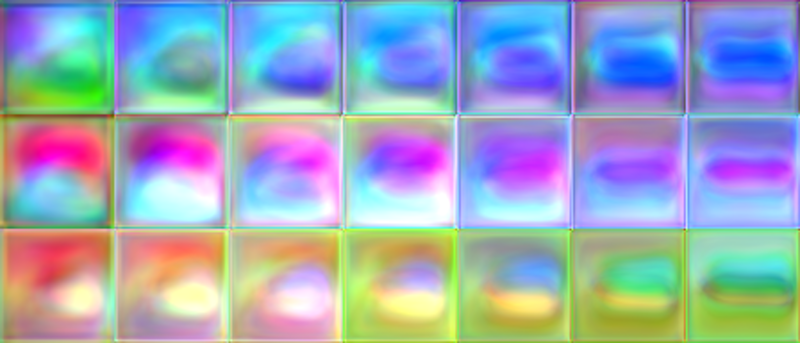
\includegraphics[width=0.45\textwidth]{figures/c4_unstable/train_samples/cos_cos/scaled_step_4_g1.png}}
    \hfill
    \subfloat[]{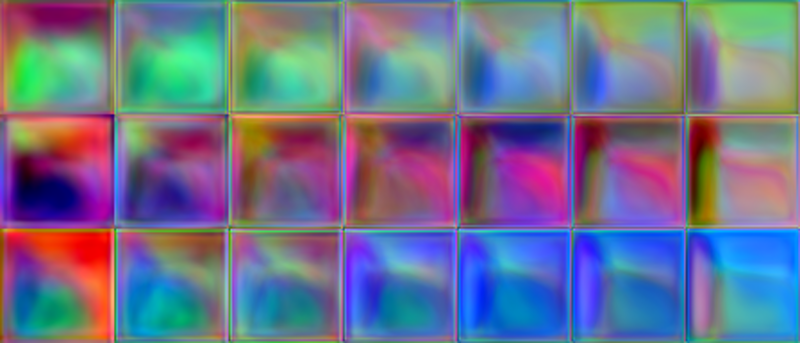
\includegraphics[width=0.45\textwidth]{figures/c4_unstable/train_samples/cos_cos/scaled_step_4_g2.png}}
    \hfill
    \subfloat[]{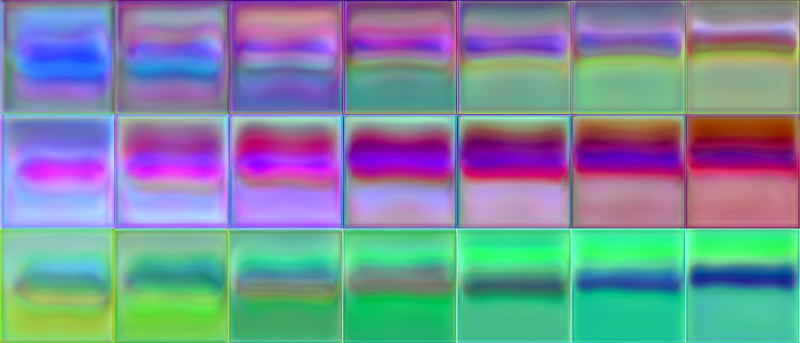
\includegraphics[width=0.45\textwidth]{figures/c4_unstable/train_samples/cos_cos/scaled_step_5_g1.png}}
    \hfill
    \subfloat[]{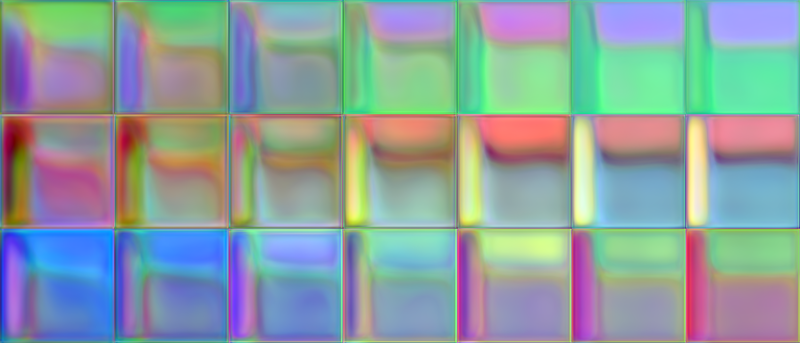
\includegraphics[width=0.45\textwidth]{figures/c4_unstable/train_samples/cos_cos/scaled_step_5_g2.png}}
    \hfill
    \subfloat[]{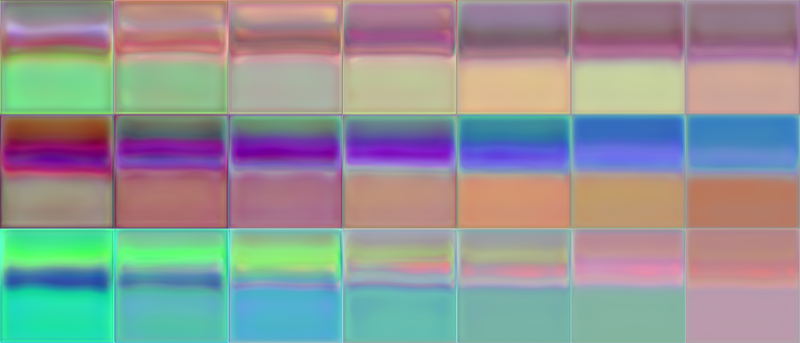
\includegraphics[width=0.45\textwidth]{figures/c4_unstable/train_samples/cos_cos/scaled_step_6_g1.png}}
    \hfill
    \subfloat[]{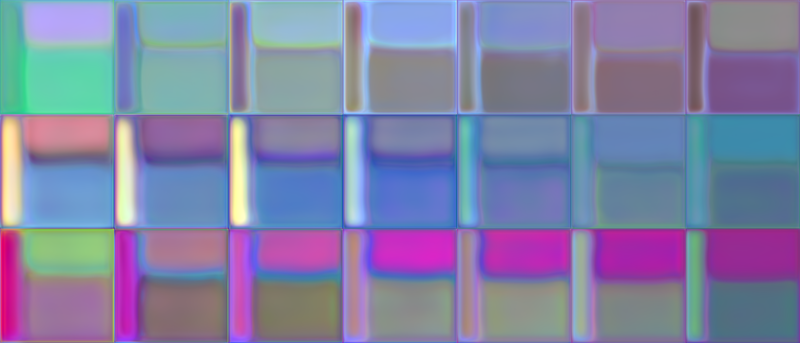
\includegraphics[width=0.45\textwidth]{figures/c4_unstable/train_samples/cos_cos/scaled_step_6_g2.png}}
    \hfill
    \caption[Training samples for two generators with cosine distance with additional colour variance loss term]{Training samples for two generators with cosine distance with additional colour variance loss term, sampled at increments of 50 iterations. The left column shows the training samples for $G_{1}$ and the right column shows the trianing samples for $G_{2}$. (a,b) Training samples at resolution 32x32 for iterations 0-300. (c,d) Training samples at resolution 64x64 for iterations 300-600. (e,f) Training samples at resolution of 128x128 for iterations 600-900. (g,h) Training samples at resolution 256x256 at iterations 900-1200. (i,j) Training samples at resolution 512x512 for iterations 1200-1500.}
    \label{fig:c3:samples-cos-cos}
  \end{figure}

  \begin{figure}[!htbp]
    \centering
    \subfloat[]{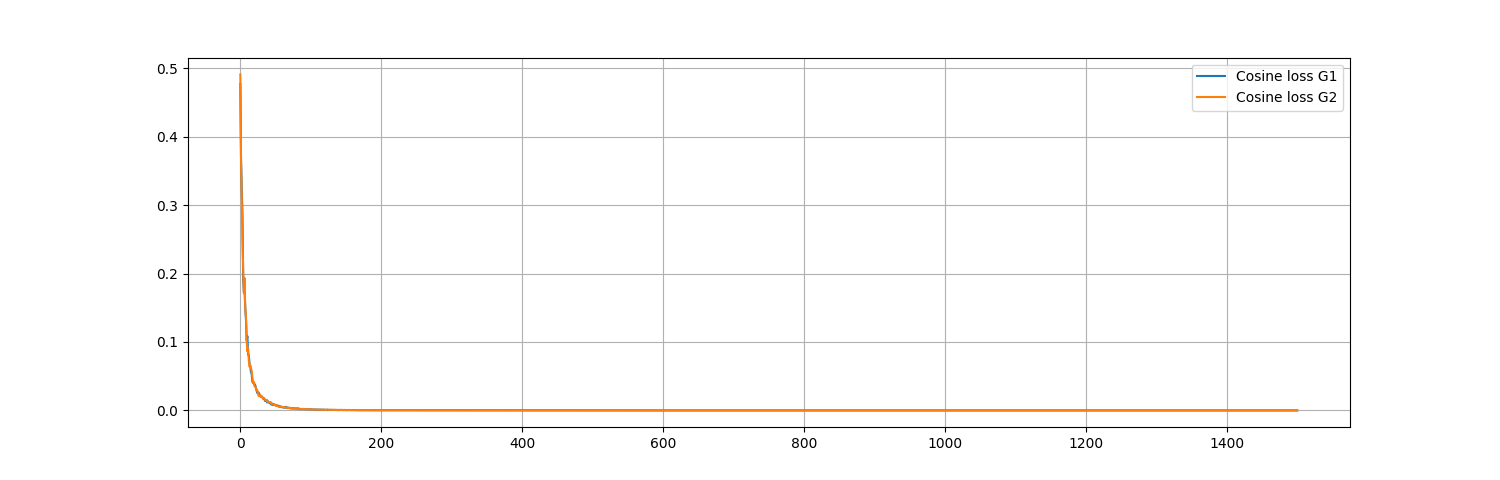
\includegraphics[width=1\textwidth]{figures/c4_unstable/train_losses/cos_cos/cosine_loss.png}}
    \hfill
    \subfloat[]{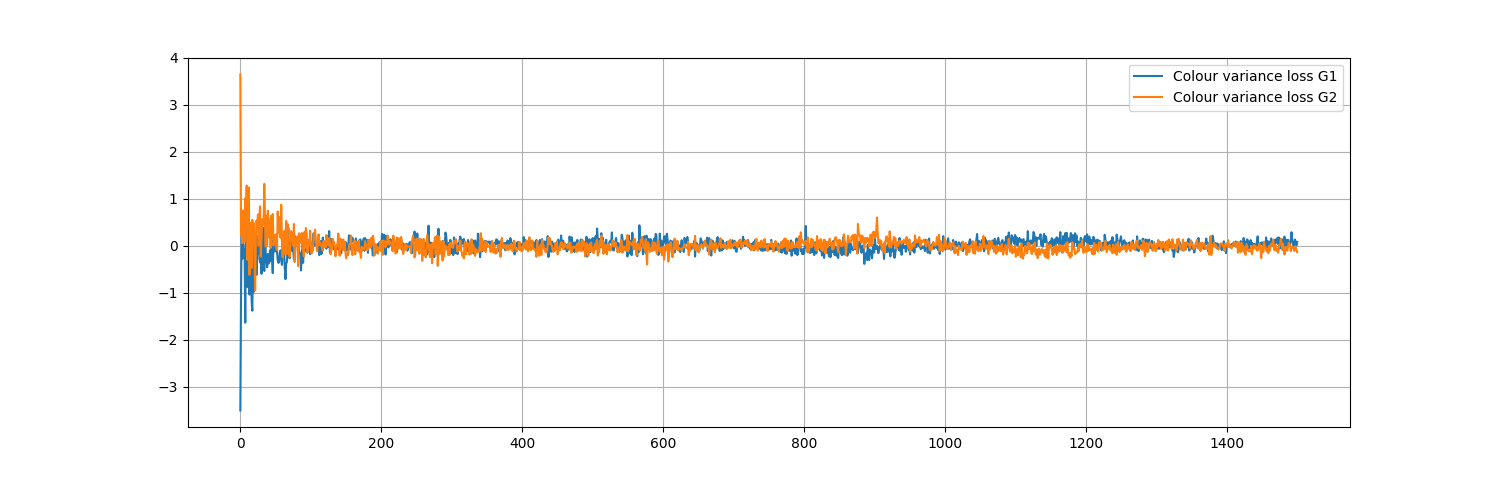
\includegraphics[width=1\textwidth]{figures/c4_unstable/train_losses/cos_cos/col_var_loss.png}}
    \hfill
    \subfloat[]{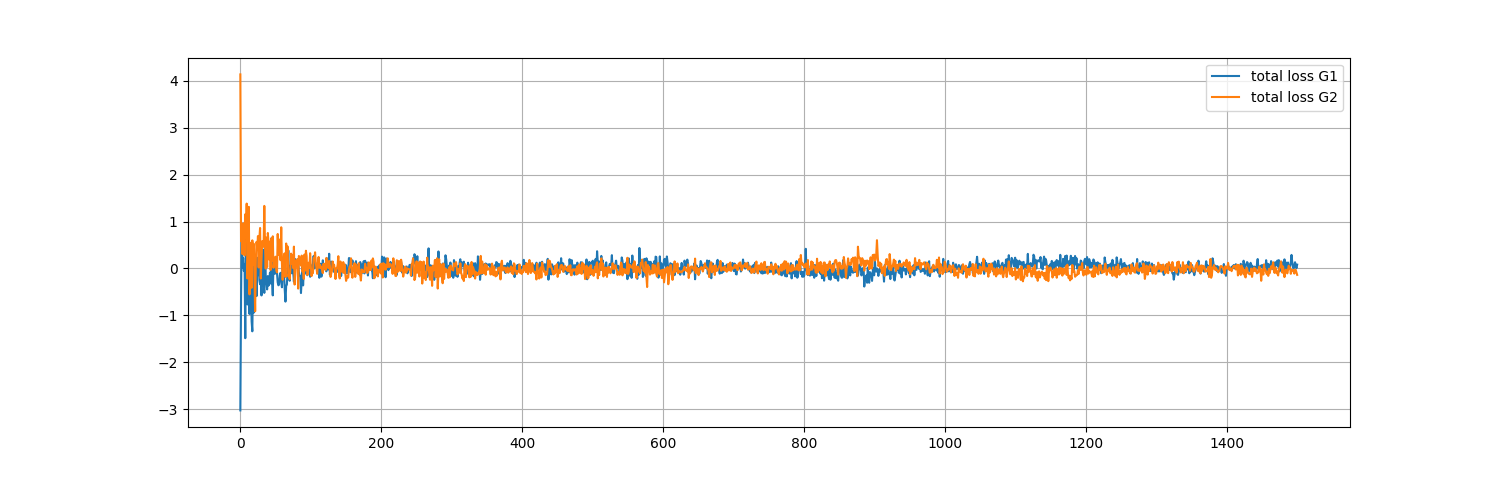
\includegraphics[width=1\textwidth]{figures/c4_unstable/train_losses/cos_cos/total_loss.png}}
    \caption[Loss plots for cosine distance training with colour variation loss term]{Loss plots for cosine distance training with colour variation loss term. (a) Cosine distance loss terms for both respective generators. (b) Colour variation loss term for both respective generators. (c) Total loss combining both terms for both respective generators. }
    \label{fig:c3:cos-cos-losses}
  \end{figure}

  \FloatBarrier

  \subsection{Euclidean distance}

\begin{equation} 
    Euclidean\ distance(x,y) = \left \lVert x - y \right \rVert_2
    \label{eq:euclid-dist}
\end{equation}

\begin{equation} 
    G_{1}\ loss = \left \lVert \vec g_{1} - \vec g_{2} \right \rVert_2 + Var(B_{g_{1}}^{c}) - Var(B_{g_{2}}^{c})
    \label{eq:g1-euclid-loss}
\end{equation}

\begin{equation} 
    G_{2}\ loss = \left \lVert \vec g_{2} - \vec g_{1} \right \rVert_2 + Var(B_{g_{2}}^{c}) - Var(B_{g_{1}}^{c})
    \label{eq:g2-euclid-loss}
\end{equation}


  \FloatBarrier

  \begin{figure}[!htbp]
    \centering
    \subfloat[]{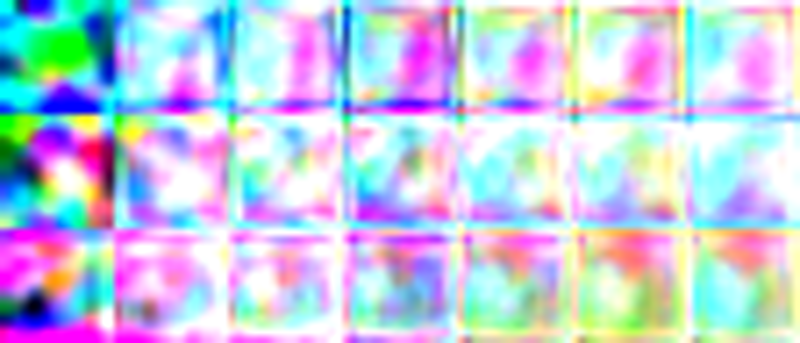
\includegraphics[width=0.45\textwidth]{figures/c4_unstable/train_samples/euclid_euclid/scaled_step_2_g1.png}}
    \hfill
    \subfloat[]{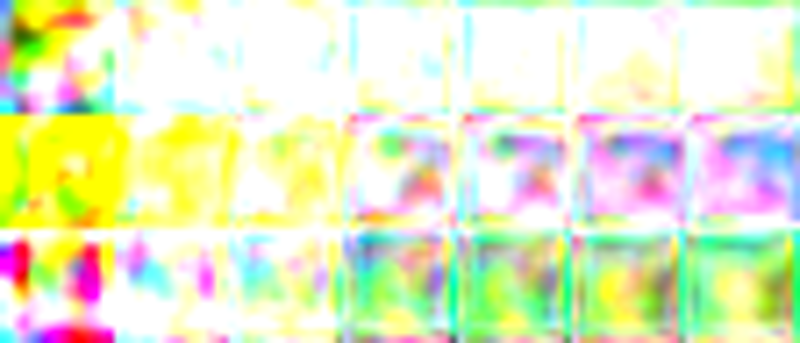
\includegraphics[width=0.45\textwidth]{figures/c4_unstable/train_samples/euclid_euclid/scaled_step_2_g2.png}}
    \hfill
    \subfloat[]{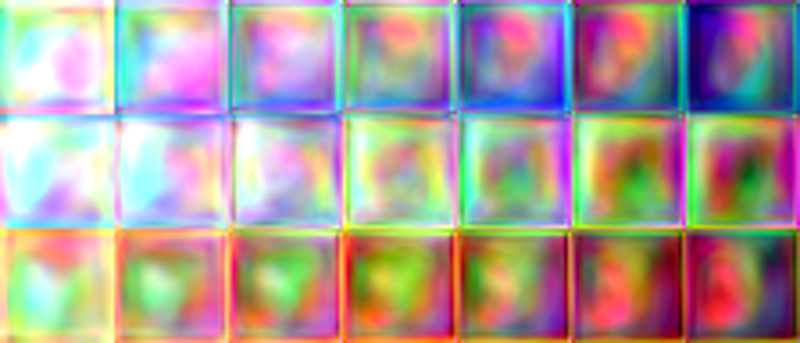
\includegraphics[width=0.45\textwidth]{figures/c4_unstable/train_samples/euclid_euclid/scaled_step_3_g1.png}}
    \hfill
    \subfloat[]{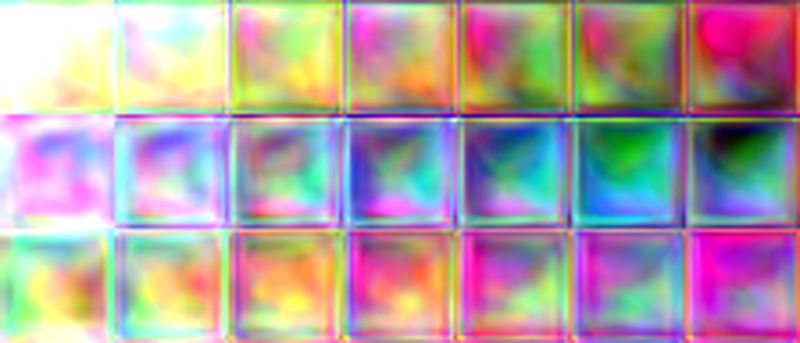
\includegraphics[width=0.45\textwidth]{figures/c4_unstable/train_samples/euclid_euclid/scaled_step_3_g2.png}}
    \hfill
    \subfloat[]{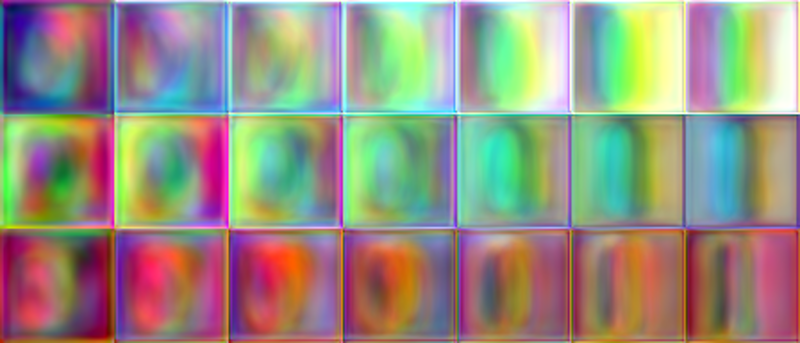
\includegraphics[width=0.45\textwidth]{figures/c4_unstable/train_samples/euclid_euclid/scaled_step_4_g1.png}}
    \hfill
    \subfloat[]{\includegraphics[width=0.45\textwidth]{figures/c4_unstable/train_samples/euclid_euclid/scaled_step_4_g2.png}}
    \hfill
    \subfloat[]{\includegraphics[width=0.45\textwidth]{figures/c4_unstable/train_samples/euclid_euclid/scaled_step_5_g1.png}}
    \hfill
    \subfloat[]{\includegraphics[width=0.45\textwidth]{figures/c4_unstable/train_samples/euclid_euclid/scaled_step_5_g2.png}}
    \hfill
    \subfloat[]{\includegraphics[width=0.45\textwidth]{figures/c4_unstable/train_samples/euclid_euclid/scaled_step_6_g1.png}}
    \hfill
    \subfloat[]{\includegraphics[width=0.45\textwidth]{figures/c4_unstable/train_samples/euclid_euclid/scaled_step_6_g2.png}}
    \hfill
    \caption[Training samples for two generators with Euclidean distance with additional colour variance loss term]{Training samples for two generators with Euclidean distance with additional colour variance loss term, sampled at increments of 50 iterations. The left column shows the training samples for $G_{1}$ and the right column shows the trianing samples for $G_{2}$. (a,b) Training samples at resolution 32x32 for iterations 0-300. (c,d) Training samples at resolution 64x64 for iterations 300-600. (e,f) Training samples at resolution of 128x128 for iterations 600-900. (g,h) Training samples at resolution 256x256 at iterations 900-1200. (i,j) Training samples at resolution 512x512 for iterations 1200-1500.}
    \label{fig:c3:samples-euclid-euclid}
  \end{figure}

  \begin{figure}[!htbp]
    \centering
    \subfloat[]{\includegraphics[width=1\textwidth]{figures/c4_unstable/train_losses/euclid_euclid/euclid_loss.png}}
    \hfill
    \subfloat[]{\includegraphics[width=1\textwidth]{figures/c4_unstable/train_losses/euclid_euclid/col_var_loss.png}}
    \hfill
    \subfloat[]{\includegraphics[width=1\textwidth]{figures/c4_unstable/train_losses/euclid_euclid/total_loss.png}}
    \caption[Loss plots for Euclidean distance training with colour variation loss term]{Loss plots for Euclidean distance training with colour variation loss term. (a) Euclidean distance loss terms for both respective generators. (b) Colour variation loss term for both respective generators. (c) Total loss combining both terms for both respective generators. }
    \label{fig:c3:euclid-euclid-losses}
  \end{figure}

  \FloatBarrier

\section{Mixing Generator Loss Functions}

\subsection{Cosine and Adversarial}

\FloatBarrier

\begin{figure}[!htbp]
    \centering
    \subfloat[]{\includegraphics[width=0.45\textwidth]{figures/c4_unstable/train_samples/cosine_euclid/scaled_step_2_g1.png}}
    \hfill
    \subfloat[]{\includegraphics[width=0.45\textwidth]{figures/c4_unstable/train_samples/cosine_adv/scaled_step_2_g2.png}}
    \hfill
    \subfloat[]{\includegraphics[width=0.45\textwidth]{figures/c4_unstable/train_samples/cosine_adv/scaled_step_3_g1.png}}
    \hfill
    \subfloat[]{\includegraphics[width=0.45\textwidth]{figures/c4_unstable/train_samples/cosine_adv/scaled_step_3_g2.png}}
    \hfill
    \subfloat[]{\includegraphics[width=0.45\textwidth]{figures/c4_unstable/train_samples/cosine_adv/scaled_step_4_g1.png}}
    \hfill
    \subfloat[]{\includegraphics[width=0.45\textwidth]{figures/c4_unstable/train_samples/cosine_adv/scaled_step_4_g2.png}}
    \hfill
    \subfloat[]{\includegraphics[width=0.45\textwidth]{figures/c4_unstable/train_samples/cosine_adv/scaled_step_5_g1.png}}
    \hfill
    \subfloat[]{\includegraphics[width=0.45\textwidth]{figures/c4_unstable/train_samples/cosine_adv/scaled_step_5_g2.png}}
    \hfill
    \subfloat[]{\includegraphics[width=0.45\textwidth]{figures/c4_unstable/train_samples/cosine_adv/scaled_step_6_g1.png}}
    \hfill
    \subfloat[]{\includegraphics[width=0.45\textwidth]{figures/c4_unstable/train_samples/cosine_adv/scaled_step_6_g2.png}}
    \hfill
    \caption[Training samples for two generators, one with cosine distance and one with adversarial loss, both with additional colour variance loss term]{Training samples for two generators, one with cosine distance and one with adversarial loss, both with additional colour variance loss term, sampled at increments of 50 iterations. The left column shows the training samples for $G_{1}$ and the right column shows the trianing samples for $G_{2}$. (a,b) Training samples at resolution 32x32 for iterations 0-300. (c,d) Training samples at resolution 64x64 for iterations 300-600. (e,f) Training samples at resolution of 128x128 for iterations 600-900. (g,h) Training samples at resolution 256x256 at iterations 900-1200. (i,j) Training samples at resolution 512x512 for iterations 1200-1500.}
    \label{fig:c3:samples-cosine-adv}
  \end{figure}

  \begin{figure}[!htbp]
    \centering
    \subfloat[]{\includegraphics[width=1\textwidth]{figures/c4_unstable/train_losses/cosine_adv/cosine_adv_loss.png}}
    \hfill
    \subfloat[]{\includegraphics[width=1\textwidth]{figures/c4_unstable/train_losses/cosine_adv/col_var_loss.png}}
    \hfill
    \subfloat[]{\includegraphics[width=1\textwidth]{figures/c4_unstable/train_losses/cosine_adv/total_loss.png}}
    \caption[Loss plots for mixed generator losses with cosine distance and adversarial loss, both with colour variation loss term]{Loss plots for mixed generator losses with cosine distance and adversarial loss, both with colour variation loss term. (a) Losses for both respective generators, $G_{1}$ is trained with Cosine distance and $G_{2}$ is trained the adversarial loss. (b) Colour variation loss term for both respective generators. (c) Total loss combining both terms for both respective generators. }
    \label{fig:c3:cosine-adv-losses}
  \end{figure}

  \FloatBarrier

\subsection{Euclidean and Adversarial}

\FloatBarrier

\begin{figure}[!htbp]
    \centering
    \subfloat[]{\includegraphics[width=0.45\textwidth]{figures/c4_unstable/train_samples/euclid_adv/scaled_step_2_g1.png}}
    \hfill
    \subfloat[]{\includegraphics[width=0.45\textwidth]{figures/c4_unstable/train_samples/euclid_adv/scaled_step_2_g2.png}}
    \hfill
    \subfloat[]{\includegraphics[width=0.45\textwidth]{figures/c4_unstable/train_samples/euclid_adv/scaled_step_3_g1.png}}
    \hfill
    \subfloat[]{\includegraphics[width=0.45\textwidth]{figures/c4_unstable/train_samples/euclid_adv/scaled_step_3_g2.png}}
    \hfill
    \subfloat[]{\includegraphics[width=0.45\textwidth]{figures/c4_unstable/train_samples/euclid_adv/scaled_step_4_g1.png}}
    \hfill
    \subfloat[]{\includegraphics[width=0.45\textwidth]{figures/c4_unstable/train_samples/euclid_adv/scaled_step_4_g2.png}}
    \hfill
    \subfloat[]{\includegraphics[width=0.45\textwidth]{figures/c4_unstable/train_samples/euclid_adv/scaled_step_5_g1.png}}
    \hfill
    \subfloat[]{\includegraphics[width=0.45\textwidth]{figures/c4_unstable/train_samples/euclid_adv/scaled_step_5_g2.png}}
    \hfill
    \subfloat[]{\includegraphics[width=0.45\textwidth]{figures/c4_unstable/train_samples/euclid_adv/scaled_step_6_g1.png}}
    \hfill
    \subfloat[]{\includegraphics[width=0.45\textwidth]{figures/c4_unstable/train_samples/euclid_adv/scaled_step_6_g2.png}}
    \hfill
    \caption[Training samples for two generators, one with Euclidean distance and one with adversarial loss, both with additional colour variance loss term]{Training samples for two generators, one with Euclidean distance and one with adversarial loss, both with additional colour variance loss term, sampled at increments of 50 iterations. The left column shows the training samples for $G_{1}$ and the right column shows the trianing samples for $G_{2}$. (a,b) Training samples at resolution 32x32 for iterations 0-300. (c,d) Training samples at resolution 64x64 for iterations 300-600. (e,f) Training samples at resolution of 128x128 for iterations 600-900. (g,h) Training samples at resolution 256x256 at iterations 900-1200. (i,j) Training samples at resolution 512x512 for iterations 1200-1500.}
    \label{fig:c3:samples-euclid-adv}
  \end{figure}

  \begin{figure}[!htbp]
    \centering
    \subfloat[]{\includegraphics[width=1\textwidth]{figures/c4_unstable/train_losses/euclid_adv/euclid_adv_loss.png}}
    \hfill
    \subfloat[]{\includegraphics[width=1\textwidth]{figures/c4_unstable/train_losses/euclid_adv/col_var_loss.png}}
    \hfill
    \subfloat[]{\includegraphics[width=1\textwidth]{figures/c4_unstable/train_losses/euclid_adv/total_loss.png}}
    \caption[Loss plots for mixed generator losses with cosine distance and adversarial loss, both with colour variation loss term]{Loss plots for mixed generator losses with Euclidean distance and adversarial loss, both with colour variation loss term. (a) Losses for both respective generators, $G_{1}$ is trained with Euclidean distance and $G_{2}$ is trained the adversarial loss. (b) Colour variation loss term for both respective generators. (c) Total loss combining both terms for both respective generators. }
    \label{fig:c3:euclid-adv-losses}
  \end{figure}

  \FloatBarrier

\subsection{Cosine and Euclidean}

\FloatBarrier

\begin{figure}[!htbp]
    \centering
    \subfloat[]{\includegraphics[width=0.45\textwidth]{figures/c4_unstable/train_samples/cosine_euclid/scaled_step_2_g1.png}}
    \hfill
    \subfloat[]{\includegraphics[width=0.45\textwidth]{figures/c4_unstable/train_samples/cosine_euclid/scaled_step_2_g2.png}}
    \hfill
    \subfloat[]{\includegraphics[width=0.45\textwidth]{figures/c4_unstable/train_samples/cosine_euclid/scaled_step_3_g1.png}}
    \hfill
    \subfloat[]{\includegraphics[width=0.45\textwidth]{figures/c4_unstable/train_samples/cosine_euclid/scaled_step_3_g2.png}}
    \hfill
    \subfloat[]{\includegraphics[width=0.45\textwidth]{figures/c4_unstable/train_samples/cosine_euclid/scaled_step_4_g1.png}}
    \hfill
    \subfloat[]{\includegraphics[width=0.45\textwidth]{figures/c4_unstable/train_samples/cosine_euclid/scaled_step_4_g2.png}}
    \hfill
    \subfloat[]{\includegraphics[width=0.45\textwidth]{figures/c4_unstable/train_samples/cosine_euclid/scaled_step_5_g1.png}}
    \hfill
    \subfloat[]{\includegraphics[width=0.45\textwidth]{figures/c4_unstable/train_samples/cosine_euclid/scaled_step_5_g2.png}}
    \hfill
    \subfloat[]{\includegraphics[width=0.45\textwidth]{figures/c4_unstable/train_samples/cosine_euclid/scaled_step_6_g1.png}}
    \hfill
    \subfloat[]{\includegraphics[width=0.45\textwidth]{figures/c4_unstable/train_samples/cosine_euclid/scaled_step_6_g2.png}}
    \hfill
    \caption[Training samples for two generators, one with cosine distance and one with Euclidean distance, both with additional colour variance loss term]{Training samples for two generators, one with cosine distance and one with Euclidean distance, both with additional colour variance loss term, sampled at increments of 50 iterations. The left column shows the training samples for $G_{1}$ and the right column shows the trianing samples for $G_{2}$. (a,b) Training samples at resolution 32x32 for iterations 0-300. (c,d) Training samples at resolution 64x64 for iterations 300-600. (e,f) Training samples at resolution of 128x128 for iterations 600-900. (g,h) Training samples at resolution 256x256 at iterations 900-1200. (i,j) Training samples at resolution 512x512 for iterations 1200-1500.}
    \label{fig:c3:samples-cosine-euclid}
  \end{figure}

  \begin{figure}[!htbp]
    \centering
    \subfloat[]{\includegraphics[width=1\textwidth]{figures/c4_unstable/train_losses/cosine_euclid/cosine_euclid_loss.png}}
    \hfill
    \subfloat[]{\includegraphics[width=1\textwidth]{figures/c4_unstable/train_losses/cosine_euclid/col_var_loss.png}}
    \hfill
    \subfloat[]{\includegraphics[width=1\textwidth]{figures/c4_unstable/train_losses/cosine_euclid/total_loss.png}}
    \caption[Loss plots for mixed generator losses with cosine distance and Euclidean distance, both with colour variation loss term]{Loss plots for mixed generator losses with cosine distance and Euclidean distance, both with colour variation loss term. (a) Losses for both respective generators, $G_{1}$ is trained with cosine distance and $G_{2}$ is trained the Euclidean distance. (b) Colour variation loss term for both respective generators. (c) Total loss combining both terms for both respective generators. }
    \label{fig:c3:cosine-euclid-losses}
  \end{figure}

\FloatBarrier

\section{Discussion}

The results from the experiments presented here show that it is in fact possible to train a generative neural network, without data, such that it produces both surprising and aesthetically interesting outcomes. 
The process described here of iterative development, observing loss functions and iteratively observing the samples generated at each time step, I was primarily looking to arrange a network configuration that had the right kind of dynamics to invoke interesting changes to the weights of the model, and in turn the generated outputs over time. 
As it is a generative system, closely observing what is being generated, and how that changes over training, seemed like the obvious way to monitor progress. 
It didn’t matter what the system was optimising towards, as long as training gradients stayed in the `sweet spot’, neither vanishing nor exploding, and the dynamics of training were in turn leading to interesting developments in the process of training. 

Maintaining gradients to be in this ‘sweet spot’ came with its challenges. 
Normally, stochasticity is present in the data, which is randomly sampled in mini-batches and optimised on using stochastic gradient descent. 
Here SGD and mini-batches were used for training, but there was no data to induce stochasticity into training. 
One of the challenges I set myself in training was to not rely on external information in training or inject any external stochastic process into training either. 
All of the stochasticity had to come the random initialisation of the network models, and from the dynamics between models in training. 
Too high a batch size was detrimental to ensuring there was enough stochasticity in training \footnote{This is not normally the case with training generative models, where the received wisdom is that the higher the batch size, the better}. 
With a very large batch size measurements would get too averaged out, and the dynamics in training would be flattened out. 

Using measurements that were constrained to within a batch, and measuring the difference between models and variation from within a single models batch became an important way of inducing dynamics in training that would lead to interesting results. 
By using slight variations of measuring distance and difference between batches, that also was able to induce some of the stochasticity needed to induce transformative dynamics in the system. 
Again, finding the right batch size was important for this and there was definitely a sweet spot of around 5 where the dynamics were just random enough to induce dynamics that quickly changed the weights of the model. 
\textbf{Expain on the impact of batch size changing over training}.

\section{Conclusion}

The work in this chapter was significant for a number of reasons, the artistic value and its impact in the artwork has already been mentioned. 
From the perspective of the narrative of this thesis though it was important for other reasons. 
This was the first breakthrough in the aim of developing a data-divergent, or more appropriately a data-agnostic way of training generative neural networks, such that they create something completely novel. 
The way this was achieved, leaning on my (relatively) significant experience of coding and training machine learning system, which I had grown to be quite comfortable with, to the degree that I could playfully experiment with the code, without anxiety, and with the ability of quickly building neural networks frameworks where gradient based learning was able to perform successfully.

A number of orthodoxies of machine learning are deliberately challenged in this work. 
The first, that data is needed to ‘learn’ or happen upon culturally relevant representations. That optimisation must be convex, that the goal of optimization must be clearly defined in a formula derived from a theory taken from statistics, physics or some branch of mathematics. 
That regularisation of training comes from the stochastic nature of data, and not from the dynamics of the models themselves. 
That high batch sizes and training for long periods is needed to produce high fidelity results. 
That the loss function needs to go down, and this needs to be observed over long periods of time.

The following chapter builds on this work, though instead of focusing on training models from scratch, I took my next experiments into fine-tuning models that had already been trained.



% \section{Old text}

% In this following approach, I took to the idea of again riffing on the GAN framework, but in this instance, replacing the data component of the framework with another generator. 
% The generators are both being optimised to have their outputs has been passed off as the other network, while the discriminator is acting in the standard adversarial fashion as a binary classifier trying to correctly classify the images from each network (See Fig 4). 

% \textbf{Figure 4: 2 Generator framework}

% Both generators in this framework are still using an adversarial loss, being optimised to trick the discriminator into making the wrong classification, while the discriminator is being optimised to make a correct classification. 
% It was clear this arrangement was an immediate improvement from the previous one, in the sense that there is no obvious failure condition where learning will instantly stop, and in this sense it more closely resembles what observes of GANs show as being one of the few learning algorithms in ML that has no defined point it is optimising towards \citep{nagarajan2017gradient}. 
% Rather, GANs exist as a dynamical system with no defined end, making it the perfect starting point for these experiments. 
% It was clear from the previous experiment that I needed some kind of dynamics between models that would produce some kind of stochastic process, in lieu of data, to generate ‘learning’ dynamics sufficient that the networks significantly diverge from the original state of random initialisation for a styleGAN model. 

% \textbf{Figure 5: Random initialised styleGAN}

% The first set of training runs produced nothing special. 
% There were definitely dynamics between the models leading to interesting changes to the model weights, clearly evident by observing the outputs at each time step (see Fig 6). 
% But ultimately, the models converged into a form of mode collapse where the network solely generated one mode of output. 

% \textbf{Figure 6: Batch after training (and over time?)}

% To deal with this issue, I started thinking of possible ways to overcome the mode collapse state of the model. 
% Though the dynamics of training were visually interesting, the goal of training a generative neural networks is to model a distribution, not a single image \footnote{with some notable exceptions, i.e. CPPNs, other ways of modelling individual images with one network}. 
% Therefore I need to find a way of pushing this system to have some kind of diversity in the outputs it was creating. In keeping with the ideas of adversarial learning where the networks play off against each other, I decided I could get the generators to compete to produce more colours than the other network in their mini-batch. 
% That way, the training dynamics are still from within the arrangements of the networks themselves, and not relying on any external input of what colours are ‘good’.

% The additional loss term added to force increased colours to be used was to measure the batch-wide variance of values for each pixel, in each channel of the tensor. 
% This term calculates the variance across the sampled batch B for the respective channel c of the tensor for the samples drawn from both generators g1 and g2, which are then subtracted from each other (depending on which loss is being calculated for which generator) to enforce a relative variance that is higher than the other model across the different channels of the sample tensor.

% \begin{equation}
%     \label{eq:variance-gan}
%     Vdiff = Var(B_{g_{1}}^{c}) - Var(B_{g_{2}}^{c})
%     \end{equation}

% This is calculated for the 4 channels of the tensor present in the sample batch. 
% The first channel is the overall batch bt, the following channels are the colour channels of the output images: red r, green g and blue b.

% \begin{equation}
%     \label{eq:total-gan}
%         Vdiff(B_{g_{1}}^{bt} , B_{g_{2}}^{bt}) + Vdiff(B_{g_{1}}^{r} , B_{g_{2}}^{r}) + Vdiff(B_{g_{1}}^{g} , B_{g_{2}}^{g}) + + Vdiff(B_{g_{1}}^{b} , B_{g_{2}}^{b}) 
%     \end{equation}

% The loss penalty was calculated for each generator with respect to the other. 
% Therefore each generator was optimised to have more mini-batch variance than the other. 
% Adding this term made a significant impact to the training. 
% The networks showed the similar behaviour of having blobs changing over time, but this time maintaining the diversity in the mini-batches (See figure 7). 

% \textbf{Figure 7: Training over time}

% When sampling the results from the final model, it is clear to see that diversity in the generator output for both models is much greater. 
% The spatial structure remains largely consistent throughout, but there is a seemingly endless variation in the colours and combinations of colours generated by the models (see next fig).

% \textbf{Figure 8: Latent interp of first model}

% The results from this experiment were surprising, to say the least. 
% My immediate reaction was to think something along the lines of “wow, that really looks like a Mark Rothko painting”. 
% This was not the goal of this work, I had no idea how the images would turn out and I had no real predefined idea in my head of what I wanted. 
% Perhaps my aesthetic judgement guided me towards developing a training system that optimises towards this in some way, but I wouldn't particularly call myself a Rothko fan. 

% Besides the resemblance to Rothko’s work, what was most striking for me was the seeming use of complementary colours in the images generated by the models \footnote{I recall a conversation I had with Professor Matthew Fuller where I showed him these images and he lamented the fact that a computer could generate something that was so tasteful.} 
% There were no mathematical theories used for determining complementary and contracting colours that the model was using, this the simple constraint of pixel-wide variance for each channel across a mini-batch. 
% One of the indirect compliments I got from this was a woman at NeurIPS who was convinced that I must have used some kind of data derived from the American colour field painting artistic movement when training the models.
